\documentclass[11pt,b5paper]{book}

% from phd template
%\usepackage[margin=20mm,top=15mm,bindingoffset=10mm,includeheadfoot,headheight=14.5pt]{geometry}
\usepackage[cam,a4,center]{crop}

\usepackage[utf8]{inputenc}
\usepackage[british]{babel}

%\usepackage{lmodern}
\usepackage{microtype}
\usepackage{graphicx}
\graphicspath{{imgs/}}
\DeclareGraphicsExtensions{.pdf,.png,.jpg,jpeg}
\usepackage{pdfpages}
\usepackage[disable]{todonotes}
\usepackage{wrapfig}
\usepackage{booktabs, tabulary, longtable}
\usepackage{rotating, multirow, pdflscape}
\usepackage[flushleft]{threeparttable}
\usepackage{xcolor}
\usepackage{framed}

% Table of contents formatting
\renewcommand{\contentsname}{Table of Contents}
\setcounter{tocdepth}{4}
\setcounter{secnumdepth}{4}

%hyperlinks
\usepackage[unicode=true]{hyperref}
\hypersetup{breaklinks=true,
            bookmarks=true,
            pdfauthor={Simone Mora},
            pdftitle={PhD Thesis},
            colorlinks=true,
           citecolor=blue,
            urlcolor=blue,
           linkcolor=magenta,
        %    pdfborder={0 0 0}
			}
\urlstyle{same}  % don't use monospace font for urls

%Pharagraph style
\setlength{\parindent}{0pt} 
\setlength{\parskip}{6pt plus 2pt minus 1pt} 
%\setlength{\emergencystretch}{3em} % prevent overfull lines 

% Headers and page numbering 
\usepackage{fancyhdr}
\pagestyle{fancy}
\addtolength{\headheight}{2.5pt}
\addtolength{\oddsidemargin}{0.7cm}
\addtolength{\evensidemargin}{-0.7cm}
\fancyhead{}				% Header flush
\fancyfoot{}
\fancyhead[LE,RO]{\thepage}	% Page number on the external side of the pages
\fancyhead[RE]{\leftmark}		% Chapter name on the right page
\fancyhead[LO]{\rightmark}	% Section name on the left page
% Improving chapter name in the header
\renewcommand{\chaptermark}[1]{%
\markboth{\thechapter.\ #1}{}}
% Improving section name in the header
\renewcommand{\sectionmark}[1]{\markright{\thesection\ #1}} 

%Hypernation
\hyphenation{UbiCollab}

%Bibliography
\usepackage[backend=bibtex,style=authoryear]{biblatex}
\addbibresource{biblio}

%Service commands
\newcommand*{\missingreference}[1]{\colorbox{red}{?#1?}}%JB
\newcommand*{\missingcitation}[1]{\colorbox{red}{?#1?}}%JB
\makeatletter
\def\@setref#1#2#3{%
  \ifx#1\relax
   \protect\G@refundefinedtrue
   \nfss@text{\reset@font\missingreference{#3}}%%JB
   \@latex@warning{Reference `#3' on page \thepage \space
             undefined}%
  \else
   \expandafter#2#1\null
  \fi}
\def\@citex[#1]#2{\leavevmode
  \let\@citea\@empty
  \@cite{\@for\@citeb:=#2\do
    {\@citea\def\@citea{,\penalty\@m\ }%
     \edef\@citeb{\expandafter\@firstofone\@citeb\@empty}%
     \if@filesw\immediate\write\@auxout{\string\citation{\@citeb}}\fi
     \@ifundefined{b@\@citeb}{\hbox{\reset@font\missingcitation{#2}}%%JB
       \G@refundefinedtrue
       \@latex@warning
         {Citation `\@citeb' on page \thepage \space undefined}}%
       {\@cite@ofmt{\csname b@\@citeb\endcsname}}}}{#1}}
\makeatother
\newcommand{\specialcell}[2][c]{%
  \begin{tabular}[#1]{@{}l@{}}#2\end{tabular}}
	% \specialcell{Date,\\duration}
	
% left align in table paragraphs
\usepackage{array}
\newcolumntype{P}[1]{>{\raggedright\arraybackslash}p{#1}}
	
% Metadata
\newcommand{\MRQ}{What are the opportunities introduced by combining reflective learning theories with sensing-based interfaces for supporting crisis training?} 
\newcommand{\RQi}{How sensing-based interfaces can be designed to enable unobtrusive experience collection during crisis work?}
\newcommand{\RQii}{How sensing-based interfaces can be designed to trigger and support reflection activities?}	
\newcommand{\RQiii}{How sensing-based interfaces for supporting reflection can be rapidly prototyped?}	
\newcommand{\Ci}{Implementation and evaluation of MIRROR Computer Supported Reflective Learning (CSRL) theory}
\newcommand{\Cii}{Knowledge about designing experience-capturing tools for crisis workers}
\newcommand{\Ciii}{Novel sensing-based interaction techniques to support re-creation and generation of work experiences in crisis training}
\newcommand{\Civ}{Knowledge about implementing prototypes to be deployed into the wild}


%-------------------------------------

\begin{document}

\includepdf[pages={1,2}]{cover.pdf}
\frontmatter
\chapter{Abstract}

Continuous training for preparedness empowers crisis workers (e.g. firefighters, paramedics) to achieve better performance and commitment in providing help to the communities struck by a nature or human-caused crisis. To achieve these goals the body of research in reflective learning provides theoretical tools to guide data-driven, collaborative reflection on work experience towards changes in behaviour. ICT support for reflective learning facilitates the process by providing technologies for capturing work experience, visualising discrepancies as reflection triggers; and by supporting sharing of learning outcomes. Yet current ICT tools do not consider the very specific, situated nature of crisis work. While data capturing tools lack interaction paradigms suitable for being used during work, visualisation tools struggle in providing the user with the context information needed to ground reflection on past work experiences and to achieve learning outcomes that are structured to be easily shared among colleagues.

The research in this thesis investigates how theory in the field of embodied and sensing-based interaction can inform the design of computer interfaces to better assist reflection practice in the case of crisis training. This thesis explores how conceptual tools from reflective learning theory can be implemented in technology tools to make the capture of work experience lightweight and pervasive, and interaction with reflection-useful information tangible, situated and playful.

The work is grounded on design science methodology. Six field studies have been performed during large physical simulations of crisis work. Exploratory studies drove eight design iterations of sensing-based interfaces. Software and hardware rapid prototyping techniques, open source and digital manufacturing tools have been largely employed. Prototypes were eventually returned to the field and tested against acceptance, usability and impact on learning. Results from evaluations were used to validate existing theories and for the development of new constructs. Commercial exploitation of the research outcomes are being discussed.

The resulting contributions add new knowledge to guide the design of novel sensing-based interfaces to support continuous training of crisis workers. To this end, it is demonstrated how conceptual tools from reflective learning theory can be mapped to technology to support the \emph{capture}, \emph{re-creation} and \emph{generation} of work experience. Seven challenges to drive the design of experience-capturing tools are provided. The challenges shed light on \emph{what} information is relevant and \emph{how} to capture relevant information and they were explored with the production of prototypes of wearable data capturing tools. Further, the thesis contributes with novel techniques derived from sensing-based interaction. The paradigms have been implemented in embodied user interfaces to reduce distraction while \emph{capturing} experience at work, to allow for \emph{re-creating} past experience situated in a physical context that provides prompts for reflection; and to allow \emph{generating} engaging and collaborative work experience by means of serious games. Building prototypes of such user interfaces requires a wide range of competencies in software and hardware engineering. Lessons learnt from the author's experience provide knowledge for the creation of designer's tools to ease rapid prototyping of sensing-based interfaces.

\chapter{Preface}

This thesis is submitted to the Norwegian University of Science and
Technology (NTNU) for partial fulfilment of the requirements for the
degree of philosophiae doctor.

The main body of doctoral work has been performed at the Department of
Computer and Information Science, NTNU, Trondheim. Professor Monica
Divitini has been the main supervisor and Babak Farshchian has been the
co-advisor.

Part of the research work was done during academic visits to foreign
institutions: the City London University and the Massachusetts
Institute of Technology.

The doctoral work is co-funded by ``MIRROR Reflective Learning at
Work'', a research project within the EU-ICT 7FP programme.

%\chapter{Acknowledgments}
\enlargethispage{\baselineskip}

Foremost, I would like to express my deepest gratitude to my supervisor Professor Monica Divitini and co-advisor Associate Professor Babak Farshchian. Your guidance and precious advices made me a better researcher and a better person. Your support and trust, always present throughout my PhD journey, make me proud. You have been an example for me, I cannot think of better supervisors to have.

I wish to thank former and current colleagues that have contributed in many ways to my work: Birgit, Ines and Alessandro for co-authoring some of the papers, Emanuele for helping with the prototyping work; my officemates Elena, Francesco and Hans for the coffee-breaks. 

I extend my gratitude to other members of the Department of Computer and Information Science for their opinions and insights; and the staff of NTNU Technology Transfer AS, in particular Marit, Silje and Kjetil, for bringing their perspective and ideas into my research. I also thank Stewart Clark for editing Part I of this thesis.

Taking part to the MIRROR project has been essential to achieve the research goals reported in this thesis. I thank all the consortium members for the productive discussions, especially Regola s.r.l and Mr.\ Gianni della Valle for arranging the field studies this research work builds on.

During part of my PhD training I was honoured to be a guest in two foreign institutions. I thank Professor Neil Maiden at the City London University for his supervision, and colleagues and friends Anja, for the teamwork; Dara, Graham, Milena, Minou, Mobina and Jacques for taking part to the evaluation of prototypes. I'm grateful to Professor Carlo Ratti at the MIT SENSEable City Lab for his lead; and colleagues and friends Professor Paolo Santi, Professor Rex Britter, Aldo, Alice, Anthony, Chris, Clara, Kris, Luis, Matteo, Matthew, Miriam, Newsha, Pierrick, Ricardo, Remi and Yuji for their amazing work.    

I am indebted to all my friends who have supported me over the last few years, those here in Norway and those in Italy. Thanks for being always there for me.

Finally, I want to express my affection to my awesome family: Lucia, Mario, Martina and Stefano, Antonella, Corrado and Federica; grandparents Benedetta and Costante. Without you all of this would not have been possible, \emph{thanks}.

\begin{flushright}
\emph{\small Simone Mora}\\\emph{\small February 26th, 2015}	
\end{flushright}



\tableofcontents
\listoffigures
\listoftables
\listoftodos
\chapter{Abbreviations}\label{abbreviations}

NTNU Norwegian University of Science and Technology

CSRL Computer Supported Reflective Learning

TEI Tangible Embodied Interaction

HCI Human Computer Interaction

WIMP Windows Icons Mouse Pointers

GUI Graphical User Interfaces

TUI Tangible User Interfaces

MAR Mobile Augmented Reality

Disaster

Emergency

Crisis

Crisis Training

Crisis Preparedness

Crisis Management

Crisis Work


\mainmatter
\mainmatter

\part[Part I]{Introduction and methods}

\chapter{Introduction}\label{introduction}

\section{Problem statement}\label{problem-statement}

This thesis is about how to improve crisis training with ICT systems. Crisis training is an umbrella term for complex, collaborative activities aiming at improving people's ability for \emph{preparedness} to human and natural-caused crises (e.g.~a flood or a terrorist attack) \autocite{Lagadec:1997js}. The term \emph{crisis} refers to a sequence of problematic events that, if left unattended, might eventually lead to a \emph{disaster}, causing huge damage and loss of lives. Disasters have a huge impact on societies, both in terms of human beings and costs. Over the last 35 years, the frequency of disasters has increased five-fold; the damage caused has multiplied approximately eight times\footnote{Source: ``Council adopts new Union Civil Protection Mechanism'' Available at: www.consilium.europa.eu/uedocs/cmsdata/docs/pressdata/en/jha/140108.pdf.}. According with the United Nation Office for Disaster Risk Reduction, over the decade 1992-2012, disasters have affected 4.4 billion people and have caused USD 2 trillion in damage worldwide\footnote{Source: The United Nation Office for Disaster Risk Reduction (http://unisdr.org)}. For this reason training for better crisis management is a priority for many countries, including those in Europe.

Crisis training focuses on teaching emergency workers (e.g.~firefighters, paramedics) how to efficiently respond to a crisis; for example by actuating coping strategies and implementing rescue procedures (crisis management). Each crisis is likely to be a specific, unpredictable event that will not take place again under the same circumstances. Training for crisis preparedness is a wicked problem, however better crisis management can positively affect everyone's lives.

There are four main approaches to crisis training: protocol training, tabletop exercises, physical simulations and serious games; on top of that real crises also offer triggers for learning \autocite{Deverell:2009fk}. In this research work we look at medium to large scale physical simulations and serious games as key training practices; aiming at advancing them with technology. Physical simulations recreate at best real crises in terms of environment (e.g. presence of debris, collapsed buildings), and in reproducing feelings experienced by crisis workers such as stress, tension, time pressure and uncertainty \autocite{Borodzicz:2002em}. Yet they are determinated by high set-up cost and the large effort required to coordinate multiple organisations and dozens of field workers. Moreover it has been observed that the impact of those events is limited by lack of technologies, for example to capture data and maintain an overview of rescue efforts \autocite{Kyng:2006he}. Otherwise, serious games trade the realism of physical simulations to provide a more lightweight training experience which can be easily reproduced frequently by single workers or teams. The ``fun'' element typical of games is added as motivator to engage workers in frequent play \autocite{DiLoreto:2012jj}. In this perspective physical simulation and serious games are are not mutually exclusive but rather complementary approaches to crisis training, providing realistic training experiences.

\emph{The research in this thesis investigates how to maximise crisis training learning outcomes during physical and serious game-based simulation of crisis work. It is based on the assumption that training practices already in place can be enhanced by combining (i) reflective, experience-based learning approaches and (ii) advances in ICT and sensing-based interaction \autocite{Zhai:2005jm}.}\todo{Reforumlate this sentence}

Experience-based learning is a powerful tool. Facilitating learning from work experience of the different roles in the field (e.g. disaster managers vs. field workers) can bring outcomes to complement traditional formal training. Learning from experience entails reflection \autocites{boud1985reflection}{Dewey:1998ug}{kolb1974toward}. Reflection on action has been a research topic since the work of Dewey \autocite{dewey1933we} that describes how we learn by comparing our expectations to new and past experience. Reflecting on action is critical in order to learn from past experience with the goal of performing better in the future \autocites{boud1985reflection}{Schon:1983ut}; and a number of tools have been developed to support reflection, as an individual or collaborative activity. Among those, the CSRL (Computer Supported Reflective Learning) model developed as part of the MIRROR project\footnote{MIRROR Project - http://www.mirror-project.eu} aims at providing guidelines to develop technology tools to support reflection. It identifies a cycle of four stages of reflection \autocite{Krogstie:2013kf}: \emph{do work}, \emph{initiate reflection session}, \emph{conduct reflection session} and \emph{apply reflection outcomes}. For each stage a number of reflection-useful activities that can be augmented with technology are provided.

In the context of crisis training, those activities can be summarised in three areas: (i) capturing work experience, (ii) re-creating work experience and (iii) generating realistic work experience. Technology provides help in different ways. Sensors can capture aspects of real or simulated work experience, including qualitative and quantitative elemtents; data which can be visualised on a interactive computer interface to provide triggers for re-evaluating an experience towards a learning outcome, or that can be used to plan new training work. Yet current technology tools do not consider the very particular, situated nature of crisis work. While data capturing tools lack interaction paradigms that are suitable to capture experience \emph{in-action}, visualisation tools struggle in providing the users with context information needed to ground  reflection \emph{on-action}. Moreover the introduction of technology is obstacled by resistances in organisations that might be reluctant to modify accustomed practices, even if unproductive \autocite{JCCM:JCCM15}.

Theories in the field of \emph{sensing-based interaction}, can inform the design of novel technologies to better assist reflective learning in crisis training. Sensing-based interaction is a trend in HCI which promotes sensing information to make human-computer interfaces, sensing-based interfaces, more effective \autocite{Zhai:2005jm}. \emph{Tangible} and \emph{embodied} \autocite{Dourish:2001vc} are two characterising traits of such interfaces. They aim at enabling interaction with digital information exploiting the affordances that everyday objects provide, rather than traditional paradigms such as keyboard, mouse or touchscreens. Using sensor-based technology, conventional objects can be augmented and turned into ``physical handles'' for digital operations \autocite{Ishii:1997ur}, linking their traditional affordances to new digital meanings. Making interaction with computers more ``physical'' allows for leveraging humans' skills for interaction with the real world \autocite{Shaer:2009fx}. This approach might be well suited for crisis fieldwork which, contrarily to traditional office work, has a strong physical and spatial connotation. In this perspective, tangible and embodied interfaces have been successfully employed to provide natural \autocite{Terrenghi:2005gq} and situated \autocite{Klemmer:2006ez} learning and increased reflection and engagement \autocite{Rogers:2006te}. ``Being able to move around in the world and interact with pieces of the world enables learning in ways that reading books and listening to words do not''. \autocite{Klemmer:2006ez}

Yet building prototypes of sensing-based interfaces, is a complex task which requires scientists to master a wide set of skills including product design, hybrid software and electronics development, as well as hardware construction and assembly. This is still a relatively new area in HCI and it is characterised by the absence of a widely established toolchain to help the prototyping work. Rather, it is characterised by fast adoption of edging technologies and a pragmatic attitude at \emph{tinkering} and \emph{thinking-thrugh-prototyping} \autocite{Klemmer:2006ez}. Considering the essential role of prototypes in the development of novel technology; developing a skillset to enable rapid prototyping of hybrid software/hardware products is essential to the accomplishment of the goals sought by this PhD work.
\begin{figure}
	[tbh] \centering 
	\includegraphics[width=0.70
	\textwidth]{better_management} \caption{Relation among the three domain of this thesis} \label{fig:topic_relation} 
\end{figure}

\section{Research methodology}\label{research-methodology}

The work in this thesis is based on \emph{design research} \autocites{Hevner:2010gc}{March:1995gm}. The work followed a \emph{user centred approach} \autocites{MAGUIRE:2001dp}{Gulliksen:2003hd}, based on exploratory studies and design work in multiple iterations.

Several qualitative research methods \autocite{robson1993real} have been adopted, including shadowing and observation of crisis worker, during field studies and interviews. Scenarios, personas and mockups aided the user-centred design work. Consistently with design research methodology, grounded on the activities of \emph{building} artefacts for a specific purpose and of \emph{evaluating} how well the artefacts perform \autocite{March:1995gm}, a number of prototyping iterations and evaluation studies have been performed.

Prototyping involved the construction of sensing-based interfaces to support reflection processes. The design of prototypes was grounded in field studies during physical simulations of crisis that I attended. Simple prototypes were initially used to build a deeper understanding of the crisis domain, where I did not have any previous knowledge. They acted as technology probes \autocite{Hutchinson:2003il} and facilitated building and understanding of the crisis domain by engaging users in focus groups. Later, multiple iterations implemented a growing set of requirements in fully working prototypes that were robust enough to be deployed during simulated rescue work.

User evaluations followed each design iteration (Figure \ref{fig:cromar}). The aim was both to assess usability of the prototypes and impact on reflection outcomes. Prototypes were evaluated both during focus groups and during large simulations of crisis response work. Results from evaluations have fed the following design iterations, and contributed in the validation of theories on reflective learning and into the development of new constructs.
\begin{figure}
	[tbh] \centering 
	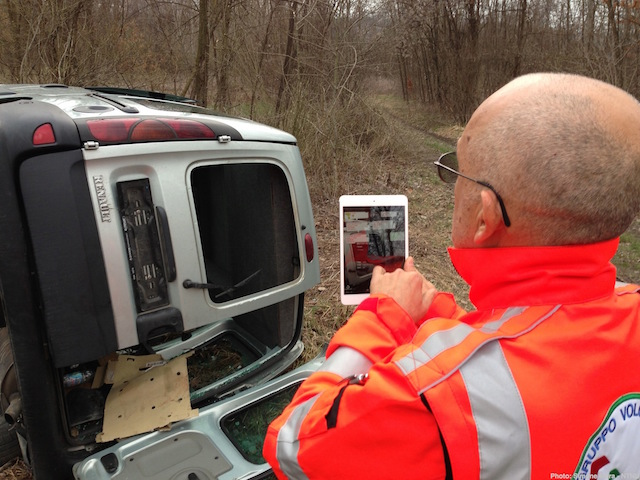
\includegraphics[width=1\textwidth]{introduction_cromar} 
	\caption{One of the evaluation field studies performed} 
	\label{fig:cromar} 
\end{figure}

\section{Research questions}\label{research-questions}

The main research question for the PhD work is:
\begin{quote}
	MRQ: \MRQ 
\end{quote}

To answer the main research question the work has been broken down into three sub-questions:
\begin{quote}
	RQ1: \RQi 
\end{quote}
\begin{quote}
	RQ2: \RQii 
\end{quote}
\begin{quote}
	RQ3: \RQiii 
\end{quote}

While the first two questions aim at investigating the design of systems to provide technology support for the tasks of \emph{capturing}, \emph{re-creating} and \emph{generating} work experience; the third question investigates how toolkits and open-source communities can ease the implementation of design ideas into prototypes.

\section{Research outcomes}\label{research-outcomes}

There are three main outcomes for this PhD work.

Seven research papers published in peer-reviewed conferences and journals explored the research questions.

Building on results reported in the papers, a body of knowledge contributing in the fields of Technology Enhanced Learning (TEL), Information Systems for Crisis Response (ISCRAM) and Tangible, Embedded and Embodied Interaction (TEI) has been developed.

Finally research contributions have been evaluated for commercial exploitation. Five \emph{Disclosure of Invention (DOFI)} have been filed for technology transfer and early contacts with the industry have been established.

\subsection{Research papers}\label{research-papers}

The research questions RQ1-RQ3 are addressed in the following research papers:
\begin{quote}
	\textbf{P1:} Mora, S., Boron, A., \& Divitini, M. (2012). CroMAR: Mobile Augmented Reality for Supporting Reflection on Crowd Management. \emph{International Journal of Mobile Human Computer Interaction}, 4(2), 88--101. 
\end{quote}
\begin{quote}
	\textbf{P2:} Mora, S., \& Divitini, M. (2014). Supporting Debriefing with Sensor Data: A Reflective Approach to Crisis Training. \emph{In Proceedings of Information Systems for Crisis Response and Management in Mediterranean Countries, ISCRAM-MED}, 196(7), 71--84. 
\end{quote}
\begin{quote}
	\textbf{P3:} Mora, S., \& Divitini, M. (2014). WATCHiT: a modular and wearable tool for data collection in crisis management and training. \emph{In Proceedings of the European Conference in Ambient Intelligence, AMI}, 8850(22), 274-289. 
\end{quote}
\begin{quote}
	\textbf{P4:} Di Loreto, I., Mora, S., \& Divitini, M. (2012). Don't Panic: Enhancing Soft Skills for Civil Protection Workers. \emph{In Proceedings of International Conference on Serious Games Development Applications, SGDA}, 7528(1), 1--12. 
\end{quote}
\begin{quote}
	\textbf{P5:} Mora, S., Di Loreto, I., \& Divitini, M. The interactive-token approach to board games. \emph{Ready for submission}. 
\end{quote}
\begin{quote}
	\textbf{P6:} Müller, L., Divitini, M., Mora, S., Rivera-Pelayo, V., \& Stork, W. (2014). Context Becomes Content: Sensor Data for Computer Supported Reflective Learning. \emph{IEEE Transactions on Learning Technologies}, PP(99). 
\end{quote}
\begin{quote}
	\textbf{P7:} Mora, S., \& Farshchian, B. A. (2010). A Unified Architecture for Supporting Direct Tag-Based and Indirect Network-Based Resource Discovery. \emph{In Proceedings of the International Conference on Ambient Intelligence, AMI}, 6439(20), 197--206. 
\end{quote}

Table \ref{tab:rq-papers-relation} shows the mapping between research papers and research questions. In addition to these papers, this PhD work has produced seven secondary conference papers. These works present incremental achievements in research that have added to the investigation of the research questions. Abstracts of the papers are included in Appendix \ref{secondary-papers}

\begin{table}
	[tbh] \centering \caption{The relation between research papers and research questions} \label{tab:rq-papers-relation} 
	\begin{tabular}
		{P{\dimexpr 0.075\linewidth-2\tabcolsep}P{\dimexpr 0.40\linewidth-2\tabcolsep}ccccccc} \toprule \multicolumn{2}{l}{Research questions} & P1 & P2 & P3 & P4 & P5 & P6 & P7 \\
		\midrule RQ1 & \RQi & & \textbullet & \textbullet & & & \textbullet & \\
		RQ2 & \RQii & \textbullet & \textbullet & & \textbullet & \textbullet & \textbullet & \\
		RQ3 & \RQiii & & & \textbullet & & \textbullet & & \textbullet \\
		\bottomrule 
	\end{tabular}
\end{table}

\subsection{Research contributions}\label{research-contributions}

The seven papers published added to the following contributions. The relation between research papers and the main topics of the research contributions is represented in Figure \ref{fig:mapping}
\begin{quote}
	\emph{\textbf{C1:} \Ci.} It includes a validation of previous theoretical models and the formulation of new constructs. 
\end{quote}
\begin{quote}
	\emph{\textbf{C2:} Knowledge about designing experience-capturing tools for crisis workers.} It defines the design space as well as design challenges for building computer-based data capturing tools. 
\end{quote}
\begin{quote}
	\emph{\textbf{C3:} Novel sensing-based interaction techniques to support re-creation and generation of work experiences in crisis training.} It describes novel user interfaces for the visualisation and manipulation of data captured from work experience. 
\end{quote}
\begin{quote}
	\emph{\textbf{C4:} Knowledge about implementing prototypes to be deployed into the wild.} It presents challenges and lessons learnt derived from the author's experience in building prototypes of sensing-based interfaces. 
\end{quote}
\begin{figure}
	[tb] \centering 
	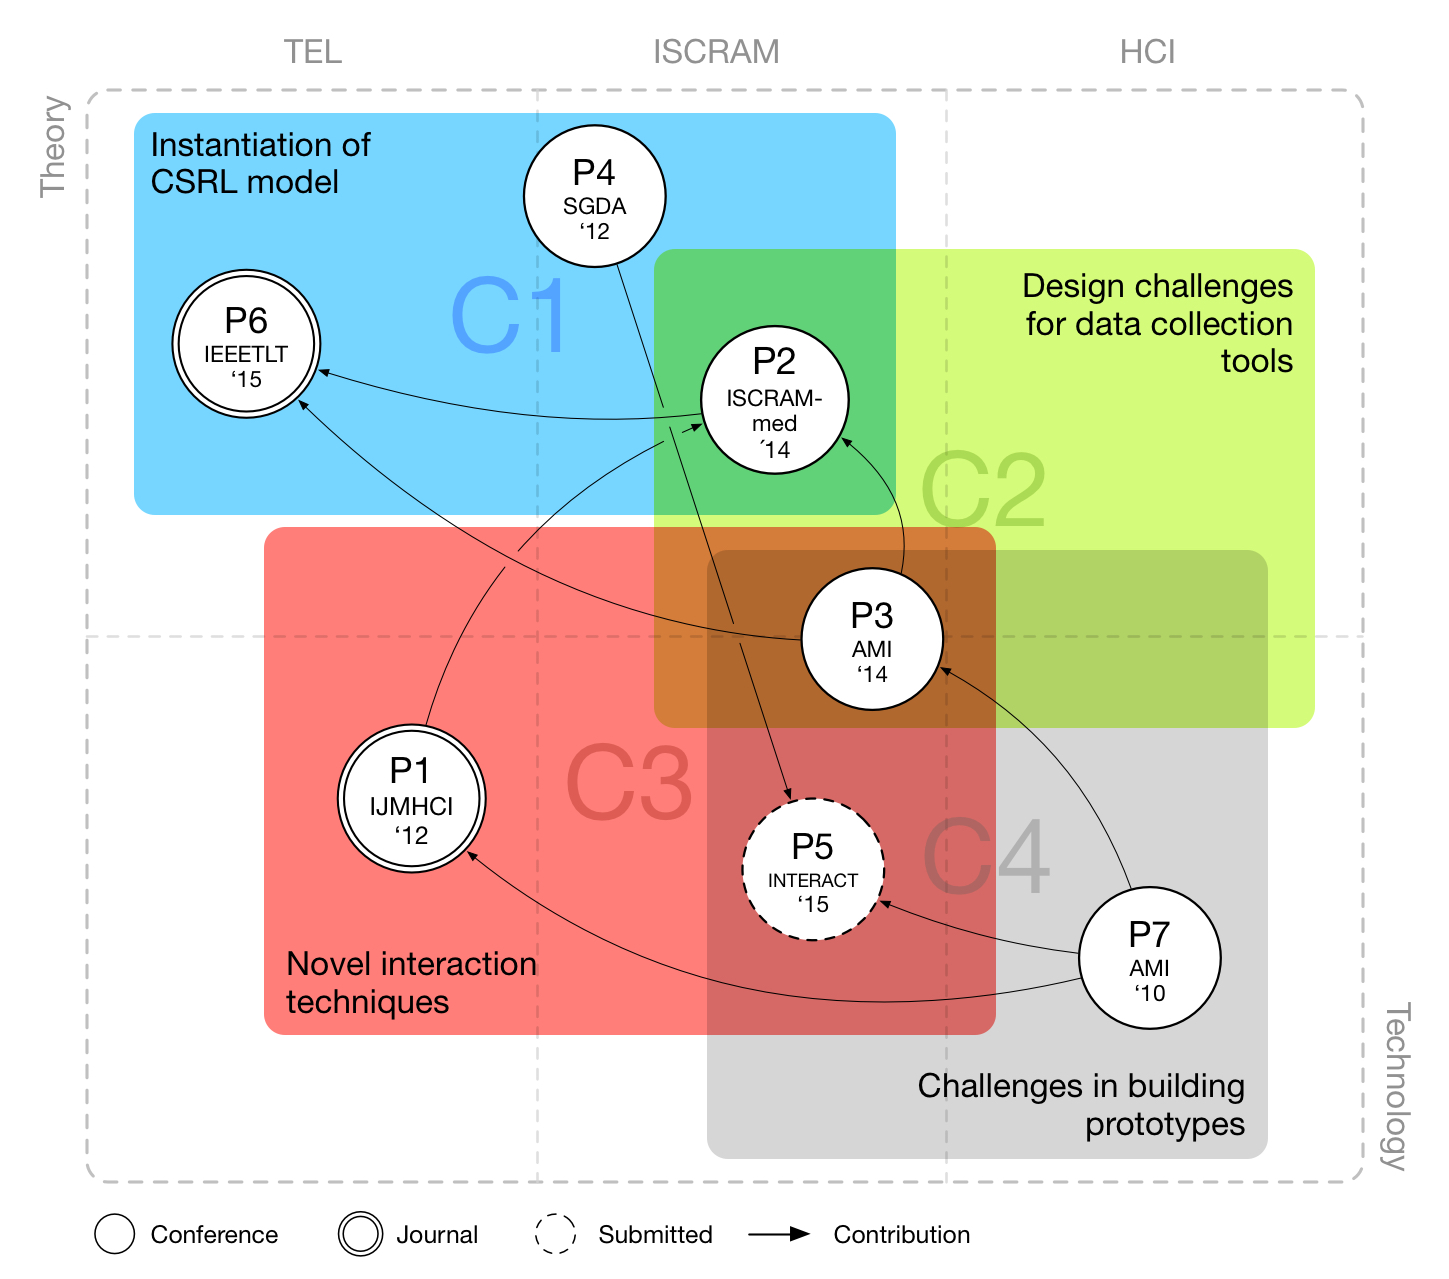
\includegraphics[width=1
	\textwidth]{papers-contributions-mapping} \caption{Research papers and the main topics of the research contributions} \label{fig:mapping} 
\end{figure}

These contributions are relevant for several research communities including Technology Enhanced Learning (TEL), Tangible Embodied and Embedded Interaction (TEI), Information Systems for Crisis Response (ISCRAM).

\subsection{Towards exploitation of research}\label{exploitation-of-research-contributions}

During the final phase of the investigation, commercial exploitation of research contributions has been investigated. The focus was on assessing efforts needed and path of actions to evolve the prototypes developed as theory demonstrator into commercial products. To this end, I co-authored five \emph{Disclosure of Invention} (DOFI): technical documents that capture the description of the technologies created and establish inventorship. DOFIs were drafted based on information published in research papers (Table \ref{tab:papers-inventions})

\begin{table}
	[tbh] \centering \caption{Relation between the inventions registered and research papers} \label{tab:papers-inventions} 
	\begin{tabular}
		{P{\dimexpr 0.05\linewidth-2\tabcolsep}P{\dimexpr 0.30\linewidth-2\tabcolsep}P{\dimexpr 0.50\linewidth-2\tabcolsep}P{\dimexpr 0.15\linewidth-2\tabcolsep}} \toprule & Authors & Invention & Research papers \\
		\midrule I1 & Mora, S., Boron, A. and Divitini, M. & CroMAR. Situated reflection and training in crisis management. & P1, P2 \\
		\noalign{\smallskip} I2 & Mora, A. and Divitini, M. & WATCHiT. Wearable data collection in crisis management and training & P2, P3 \\
		\noalign{\smallskip} I3 & Di Loreto, I., Mora, S. and Divitini, M. & ``Don’t Panic!'' A serious game for enhancing soft skills for Civil Protection workers & P4, P5 \\
		\noalign{\smallskip} I4 & Mora, S., Di Loreto, I. and Divitini, N. & Anyboard: a platform for creating and play digital board games & P5 \\
		\noalign{\smallskip} I5 & Mora, S. and Divitini, M. & TILES Toolkit. Building seamless interfaces between people and the Internet of Things & P3, P5 \\
		\bottomrule 
	\end{tabular}
\end{table}

Disclosure of inventions were filed at the NTNU Technology Transfer Office\footnote{NTNU Technology Transfer AS - http://www.tto.ntnu.no}, a business incubator affiliated with NTNU, and in accordance with Norwegian law\footnote{In accordance with ``Act respecting the right to employees' inventions 17.4-1970'', and NTNU's internal Guidelines for innovation}. They were used by technology transfer managers to assess patent applicability and establishment of commercial activities. To this effort, I presented the research outcomes to several representatives from the industries working in the emergency management field, raising positive and supportive feedbacks. In November 2014 I was granted by NTNU Discovery \footnote{NTNU Discovery - http://ntnudiscovery.no} a NOK 150.000 (about USD 22.000) seed fund for financing further commercial exploration of the research results after the PhD completion.

\section{Context of the work}\label{context-of-the-work}

The research presented in this thesis is framed within the EU-funded (IST-FP7) project MIRROR\footnote{MIRROR Project - http://www.mirror-project.eu}. The objective of MIRROR is to empower and engage employees to reflect on past work performance and personal learning experience in order to learn in “real-time” and to creatively solve pressing problems. MIRROR is to help employees to increase their level and breadth of experience significantly within a short time by capturing the experience of others.  

As an associate researcher of MIRROR I took part in shaping the results of the projects by designing and implementing ICT systems, writing deliverables and attending project meetings. Thanks to MIRROR I cooperated with crisis worker associations to run field studies. I also benefited from discussions, joined works and co-authored publications with members of the consortium. After the project final review in September 2014, MIRROR has been graded as ``Excellent'' by the EU Commission.

During the PhD I was a visiting fellow to two foreign institutions: \emph{City London University}\footnote{City London University - http://city.ac.uk} in London (UK), where I was supervised by professor Neil Maiden; and \emph{MIT SENSEable City Lab}\footnote{MIT SENSEable City Laboratory - http://senseable.mit.edu} in Boston, MA (USA), under the supervision of professor Carlo Ratti. The purpose of the two visits was to investigate whether the technologies developed during the PhD could be generalised to application domains outside crisis training. A summary of the activities performed as visiting fellow is provided in Appendix \ref{abroad}.

I also co-advised the thesis work of eight master's students who have contributed to the development of prototypes. One of them co-authored P1.

\section{Structure of the thesis}\label{structure-of-the-thesis}

The thesis is composed by two parts:

\begin{itemize}
	\item \textbf{Part I} presents the introduction to this work. It gives on overview of the background, the methods used, the results achieved and the contributions provided by the thesis.
	\item \textbf{Part II} contains seven research papers that added to the results of this thesis
\end{itemize}

The rest of \textbf{Part I} is organised as follows:

\begin{itemize}
	\item \textbf{Chapter \ref{crisis}} introduces the crisis domain providing an overview on scenarios, activities and roles; and presenting debriefing as a tool for experiential learning.

	\item \textbf{Chapter \ref{csrl}} describes relevant background theory on reflective and experience-based learning with focus on describing the Computer Supported Reflective Learning model adopted as theoretical underpinning of this research work.

	\item \textbf{Chapter \ref{interaction}} presents relevant background theory in sensing based-interaction, motivating the use of that category of applied to reflective learning.

	\item \textbf{Chapter \ref{research}} depicts the research strategy and approach adopted by this PhD work, giving overview of the user studies conducted and prototypes built.

	\item \textbf{Chapter \ref{results}} summarises the results for the research papers.

	\item \textbf{Chapter \ref{contributions}} outlines the contribution of this thesis and their relations to the research papers.

	\item \textbf{Chapter \ref{evaluation}} proposes an evaluation of the work done.

	\item \textbf{Chapter \ref{conclusions}} concludes the thesis and sketches out future research and innovation work.

	\item \textbf{Appendix \ref{secondary-papers}} summarises secondary research papers that were written during the research fellowship.

	\item \textbf{Appendix \ref{abroad}} outlines research done during academic visits in foreign institutions.

	\item \textbf{Appendix \ref{toolkits}} includes a benchmark of hardware toolkits for rapid prototyping which has been used to select the specific tools used to implement the prototypes in this PhD. 
\end{itemize}

\textbf{Part II} contains the seven research papers in full length

\chapter{The case of crisis training}\label{crisis}

\todo[inline]{Revision 5}

In this chapter I provide an overview on crisis training, crisis preparedness and management, highlighting how reflection can improve learning outcomes.
\begin{figure}
	[h!] \centering 
	\includegraphics[width=1
	\textwidth]{3steps} \caption{Three stages to better deal with a crisis} \label{fig:three-stages} 
\end{figure}

\todo{delete it?}

\section{Crisis management}\label{crisis-management}

The terms \emph{crisis}, \emph{emergency} and \emph{disaster} are often used as synonyms. They deal with events that belong to the ``un-ness'' category: unexpected, undesirable, unimaginable, and often unmanageable situations \autocites{Boin:2007wt}{hewit}. In this space made up of both foreseeable and unexpected elements, crisis management works at anticipating what can be predicted in order to minimise the unforseen\footnote{Source: http://emergency-planning.blogspot.it}.

In this thesis the term \emph{crisis} refers to a single or sequence of problematic events that may lead to a dangerous situation, whether that is an \emph{emergency} or a \emph{disaster}. While an emergency is an episode that requires immediate attention, but usually on a small scale, it can turn in a disaster if left unattended. For example expected heavy rainfall could lead to several emergencies (e.g.~car crashes, flooded bridges) and might eventually turn into a disaster (e.g. massive flooding or a hurricane). Disaster can be caused by nature or humans and might or might not show early signals that allow the disaster to be avoided or mitigated. Disasters have a huge impact on societies, in terms of loss of human lives and costs. Over the last 35 years, the frequency of disasters has increased five-fold and the damage caused has multiplied by approximately eight times\footnote{``Council adopts new Union Civil Protection Mechanism'' Available at: www.consilium.europa.eu/uedocs/cmsdata/docs/pressdata/en/jha/140108.pdf.}. Over the decade 1992-2012, disasters have affected 4.4 billion people and have caused USD 2 trillion USD in damage worldwide\footnote{Source: The United Nation Office for Disaster Risk Reduction (http://unisdr.org)}.

Yet, although crises are getting more frequent, people's ability to deal with adverse events, \emph{crisis management}, is also growing \autocite{Boin:2009bv}. Crisis management involves a set of collaborative inter and intra-organisation activities to respond to a crisis. Examples of typical roles and activities deployed are: police forces to constrain access to the crisis scene, firefighters to explore and map undisclosed areas, dog handlers to search for the injured, paramedics to activate triage and hospitalise the wounded; fellow citizens to report information and stay out of danger.

Activating effective crisis management strategies can avoid or reduce the extent of an emergency or a disaster, save human lives and reduce the cost of recovery. For this reason improving crisis management practices, hereafter \emph{crisis training} is a priority for many European countries \footnote{``Council adopts new Union Civil Protection Mechanism'' Available at: www.consilium.europa.eu/uedocs/cmsdata/docs/pressdata/en/jha/140108.pdf.}. Providing better crisis management is not easy task. This is due to the nature of crisis work as a complex, inter-organisational activity, often without a clear start or end, and involving many different roles.

\section{Crisis preparedness}\label{crisis-preparedness}

The effort of providing better crisis management is also known as \emph{crisis preparedness}. It is a collective activity which involves fellow citizens, crisis workers and institutions at multiple levels. Getting prepared to a crisis is a continuous process focusing on two areas, \emph{prevention} and \emph{response} \autocite{Deverell:2009fk}

\begin{figure}
	[h!] \centering 
	\includegraphics[width=1
	\textwidth]{crisis_timeline} \caption{Phases of a crisis} \label{fig:phases} 
\end{figure}

\textbf{Prevention} refers to activities aiming at avoiding a crisis; e.g.~mitigating risks by monitoring the environment and raising awareness in the population about how to recognise early warnings.

\textbf{Response} is concerned with getting ready to promptly react when a crisis occurs, in order to be able to mitigate it so that there is as little damage as possible and to reduce its impact on the population. It includes activities related to protocol formalisation and training of crisis workers.

Crisis workers are trained volunteers and professionals to provide help to the people in need; for example firefighters, police, paramedics. Training of crisis workers, hereafter \emph{crisis training}, is a critical activity to improve crisis management because it deals with the ability of people to react to a crisis and reduce the risks of the same turning into an emergency or disaster. As matter of fact, previous research has shown that the outcome of a disaster is highly correlated with preparation and training prior the beginning of the crisis \autocite{Asproth:cb}.

Different approaches and activities related to \emph{crisis training} are described in the next section.

\section{Crisis training}\label{crisis-training}

Four approaches to crisis training have been identified: protocol training, tabletop exercises, physical simulations and serious games. They share the goal to produce learning outcomes towards better crisis management practice. The presented approaches are not mutually exclusive but rather complementary. They are the expression of a trade-off between adding realism to the training experience and costs (Figure \ref{fig:training-activities}).

\begin{figure}
	[h!] \centering 
	\includegraphics[width=1
	\textwidth]{training_examples} 
	\caption{Cost and realism in different training activities} 
	\label{fig:training-activities} 
\end{figure}

\textbf{Protocol training} - It is a formal learning activity related to teaching of procedures, protocols and best practice. This is often the first type of training given to newcomers, e.g.~by means of a crisis management course.

\textbf{Tabletop exercises} - Often performed at the strategic level, it usually involves disaster managers to gather together and talk through a simulated disaster. There is usually little realism in a tabletop exercise\footnote{source: \url{http://www.epa.gov/watersecurity/tools/trainingcd/Pages/exercise-menu.html}}: equipments are not used, resources are not deployed in space and time constraints are not introduced. Tabletop exercises usually run for a few hours, the limited scale of the exercises make them a cost-effective tool to validate plans and activities.

\textbf{Physical simulations} - They are large-scale events that try to recreate as much as possible events and context from real crises, in terms of environment, tasks and challenges, stress and emotions. Simulated crisis events can run for days, they take place on-location using, as much as possible, equipment and personnel that would be deployed on a real event. Simulations involve a wide range of roles from disaster manager, to team leaders and field workers. They are high cost events and for this reason are run sporadically; it is therefore important to maximise their training outcomes.

Simulations usually take place in remote areas unaccessible to the public, which are set up to recreate harsh conditions like the presence of debris, flooded terrains, fire ashes and broken cars. In this setting, volunteers impersonating the injured to be rescued are located in places undisclosed to the trainees (Figure \ref{fig:simulation-phases}-left).
\begin{figure}
	[tbh] \centering 
	\includegraphics[width=1
	\textwidth]{simulation_phases} \caption{Different phases of a simulation, setup (left), work (centre), debriefing (right). Pictures were taken during field studies performed by the author.} \label{fig:simulation-phases} 
\end{figure}

A typical training session includes \emph{briefing}, \emph{simulation} and \emph{debriefing} phases. During briefing the esercise manager describes the settings, and assigns duties to the teams. During simulation workers implement rescue procedures (Figure \ref{fig:simulation-phases}-centre). The work involves cooperation among: police forces, to handle traffic and fence the operational area, firefighters to explore and secure undisclosed areas, civil protection workers to build field hospitals, dog handlers to search for survivors and teams of paramedics to activate triage, treat the injured and transportation to the nearest field hospital. A collaborative debriefing of the events, with focus on time of completion of procedures and issues that might have been arisen during the practice, concludes the simulation (Figure \ref{fig:simulation-phases}-right).

During this PhD work the author performed a six field studies during physical simulations. A list of the studies and methods adopted is given in Chapter \ref{research}.

\textbf{Serious games} - They aim at teaching useful skills for crisis management leveraging the ``fun'' aspect of games as a motivator to play repeatedly and gain multiple perspectives \autocite{DiLoreto:2012bj}. Rather than seeking to teach \emph{hard skills} like protocols and best practices, serious games work best at enhancing \emph{soft skills} e.g.~communication styles, stress management and coping strategies \autocite{Sagun:2009ks}. Those skills are useful both for prevention and for response to a crisis. Serious games bridge the gap between tabletop exercises and physical simulations: they are more realistic than the former yet without the huge costs of the latter. They can be played multiple times, both by individuals and collaboratively by teams. An ecology of serious games can address a variety of roles and tasks: being a lightweight training tool, each game can be tailored on a specific learning objective. Serious games for crisis training range from board game to highly immersive virtual environments, for a review see \autocite{DiLoreto:2012bj}.

While the first approach presented relies on formal learning (e.g.~classroom teaching), the other approaches can benefit from \emph{experiential learning} \autocite{kolb1984organizational} techniques; being the training experience focused on doing some extent of real work.

\subsection[Experiential learning]{Experiential learning, one of the sought-after outcomes of crisis training}\label{experiential-learning-one-of-the-sought-after-outcomes-of-crisis-training}

Experiential learning is one of the sought outcomes of crisis training. It is an informal learning approach that makes use of work experience and reflection in order to achieve learning outcomes \autocite{kolb1984organizational}. Although learning by experience and lesson drawing are still quite unexplored areas of crisis management \autocites{Lagadec:1997js}{Boin:2007wt}{Stern:1997eb}, the important role of \emph{experience} in crisis training, as means for achieving organisational learning, is widely acknowledged.

Experience gathered during real and simulated crises can be used to achieve a learning outcome \autocite{Deverell:2009fk}, which may occur ``when experience systematically alters behaviour or knowledge'' \autocite[p.233]{Schwab:2007iw}. Larsson \autocite{Larsson:2010jr} highlights how past experience (e.g.~from an earlier training event) can hold knowledge useful for managing a new crisis for example to correct mistakes done in the past: ``Personal and group experiences, together with exercises, seem to be the two most important forms of learning'' \autocite[p.714]{Larsson:2010jr}. As stated by Hillyard \autocite*{Hillyard:SYlJRQLN}, ``...learning together from an event in order to prevent, lessen the severity of, or improve upon responses to future crises''. The correct action to take often can only be derived from experience, e.g.~handling of the events in similar situations.

Yet, learning from crisis work experience is not easy. While learning during a crisis, or \emph{intra-crisis}, is very difficult due to time pressure, stress and demands for rapid action \autocite{Deverell:2009fk} and because learning is typically a retrospective exercise \autocite{jasanoff1994learning}; \emph{inter-crisis} learning, before and after a crisis event, is also challenging. Moynihan \autocite*{Moynihan:2008gq} identifies ten barriers to effective crisis learning. Among those the high consequentiality of crises makes experiential learning costly \autocite{LaPorte:1991gk}, moreover the specificity of each crisis event makes hard to apply learning outcomes from one crisis to another.

\emph{Therefore, how work experience can produce a learning outcome? And what are those learning outcomes?}?

Work experience can be turned into new knowledge thanks to the reflective practice. Reflecting on action allows workers to learn from past experience with the goal of performing better in the future \autocites{boud1985reflection}{Schon:1983ut}. In addition, sensing-based interfaces can augment the reflective practice, for example providing sensors for capturing different aspects of experience, user interfaces to facilitate the practitioner in reflecting upon information captured and infrastructures to share data and reflection outcomes among practitioners. The common denominator is that technology can add realism to exercises, in order to re-create experiences that are as close as possible to real crisis, and allow trainees to experience emotions (e.g.~stress) of a similar nature and intensity as the ones experienced under a real emergency \autocite{MacKinnon:2012wz}. Adding realism to the training experience is recognised to be a key for achieving learning outcomes \autocite{Asproth:2013vs}.

In the remaining of this thesis, theoretical frameworks presented in the next chapter describe how to promote reflection by identifying relevant \emph{cycles} of learning activities. Chapter \ref{interaction} describes how those activities can be augmented by sensing-based technologies. 

\chapter[Theoretical underpinning:\\ Computer Supported Reflective Learning]{Theoretical underpinning: Computer Supported Reflective Learning}\label{csrl}

\todo[inline]{Revision 5}

In order to provide information about the design of technology to support experiential learning in crisis training, I adopted the Computer Supported Reflective Learning model (hereafter CSRL model) developed by the MIRROR project. The model identifies the requirements to design technology to support reflective learning \autocite{Krogstie:2013kf}. The CSRL model has worked as theoretical underpinning for the development of sensing-based technologies presented in this PhD work, providing a language for guiding the understanding of reflection and drafting requirements for the technology.

After a brief introduction about theories in the field of reflective learning, I describe the CSRL model and how it can be applied to the development of technology. In the following I will use the terms \emph{reflective learning} and \emph{reflection} as synonyms.

\section{The reflective practice}\label{reflection}

Boud \autocite*{boud1985reflection} defines reflective learning as ``a generic term for those intellectual and affective activities in which individuals {[}\ldots{}{]} explore their experiences in order to lead to new understandings and appreciations'', it is both an individual and collective mental process that turns past experiences into new knowledge. This is also in line with the work of Sch\"on \autocite*{Schon:1983ut} who further distinguishes between \emph{reflection-in-action} and \emph{reflection-on-action}.

Reflection consists of a three-steps process during which the learner re-evaluates her experiences inspecting behaviours, ideas and feelings; eventually deriving conclusions and lessons learned to that guide future behaviour (Figure \ref{fig:boud-model}). The process can be iterated multiple times and might influence the learner's behaviour only in the long term.

\begin{figure}
	[tbh] \centering 
	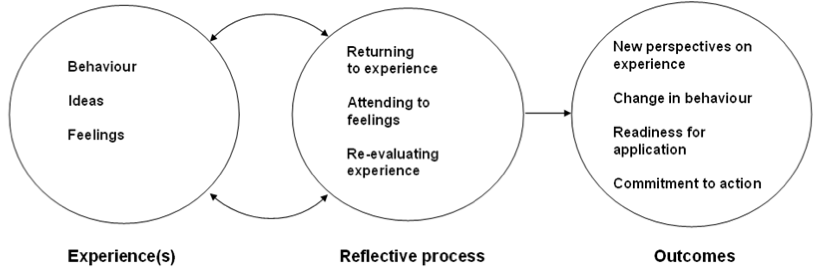
\includegraphics[width=1
	\textwidth]{boud} \caption{The reflection process according with Boud. Figure adapted from \protect\autocite{boud1985reflection}} \label{fig:boud-model} 
\end{figure}

A key aspect in making a reflective process to happen is the presence of triggers. Triggers are unexpected situations, for example disturbances and perception of uncertainty; but also positive situations like a surprising success. In general, reflection seems to be triggered by awareness of the discrepancy between expectations and the current experience. Reflection might be triggered by an external event or agent (external trigger/accident) or might develop from one's own thinking of a whole series of occurrences over time (internal trigger). Reflection can occur incidentally or intentionally, but in both cases it is a conscious evaluation of an experience. Furthermore people can learn not only from their own experiences, but also from other's experiences directly or indirectly (for example by observing and reflecting on other's actions).

Similar to the work of Boud, Kolb describes experiential learning as a cyclic process named ``The Kolb Cycle'' (Figure \ref{fig:kolb-model}).

\begin{figure}
	[tbh] \centering 
	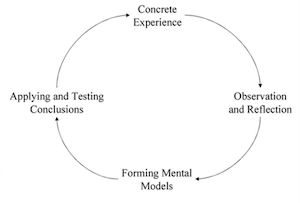
\includegraphics[width=1
	\textwidth]{kolb} \caption{"The Kolb cycle", a model of experiential learning. Figure adapted from \protect\autocite{kolb1984organizational}} \label{fig:kolb-model} 
\end{figure}

According with Kolb \autocite*{kolb1984experiential} reflection is a process that involves not only reinterpreting existing experiences, but also initial perception and interpretation of the raw experience.

For a description of other existing theories in reflective learning see \autocite{WoodDaudelin199636}.

\subsection{Collaborative reflection during debriefings}\label{debriefing-crisis-management-work-an-example-of-collaborative-reflection}

An example of collaborative reflection in crisis management is \emph{debriefing}. As outlined by Boud et al. \autocite*{boud1985reflection} debriefing is a form of collaborative reflection because during debriefings a re-evaluation of experience takes place, with explicit attention to emotions, ideas and behaviour.

Debriefing involves ``reviewing a difficult episode from a constructive point of view \ldots{} the goal is to extract fundamental lessons learned from the way the event was handled'' \autocite{Lagadec:1997js}. It is a collaborative activity involving multiple roles and it is usually performed after a (real or simulated) crisis work experience. 

Figure \ref{fig:debriefing-example} shows one of the debriefing observed during the user studies reported in Chapter \ref{research}. After a 3-day physical simulation of crisis management operations, the chief manager discusses with team leaders and field workers what went wrong and how to avoid the same issues in the future. Technology is used to visualise the location of operations on a digital map. Data were previously manually entered during the training event.

\begin{figure}
	[tbh] \centering 
	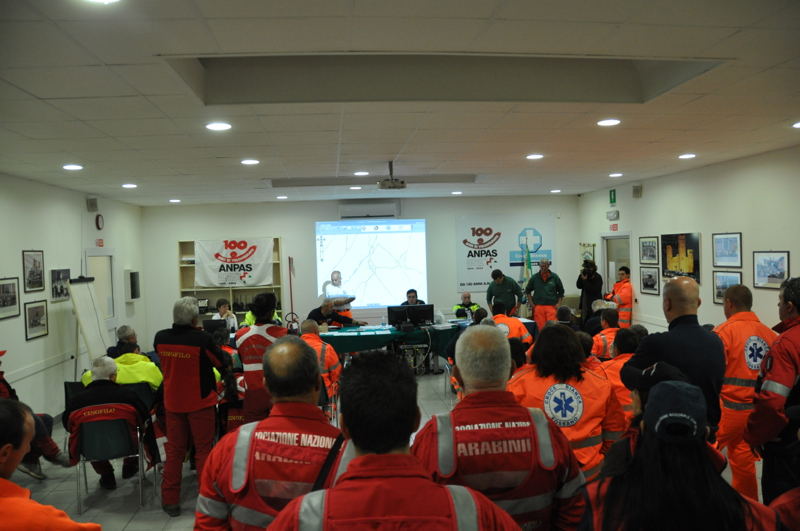
\includegraphics[width=1
	\textwidth]{debriefing} \caption{A debriefing after a physical simulation of crisis management observed by the author} \label{fig:debriefing-example} 
\end{figure}

The outcome which debriefing seeks to obtain is lesson drawing. Previous work experience provides a good source of lesson-drawing which may potentially affect managing, planning and training for future crises. Yet lessons-drawing is often one of the most neglected aspects of crisis management \autocites{Lagadec:1997js}{Stern:1997eb}. The introduction of debriefing into crisis organisations often meets resistance \autocite{Lagadec:1997js}. This might be due to lack of commitment, costs, but also the lack of technologies to make the debriefing more effective.

\section{Computer Supported Reflective Learning (CSRL), a model}\label{computer-supported-reflective-learning-a-model}

Building on the presented theories and on empirical studies, the MIRROR project has iteratively developed a model for Computer Supported Reflective Learning (CSRL model). The model has been designed to identify requirement, design and implement technology to support for reflective learning \autocite{Krogstie:2013kf}. Rather than providing formal guidelines or pre-defined processes, the model helps to understand and analyse reflection in the workplace and it suggests how technology can support reflective practice.

Following the work of Boud et al. \autocite*{boud1985reflection} the model considers reflective learning as ``the conscious re-evaluation of experience for the purposes of guiding future behaviour {[}\ldots{}{]} as reflection transforms experience from work into knowledge applicable to the challenges of daily work'' \autocite{Krogstie:2013kf}. The model specifically addresses reflection in the workplace with \emph{work} and \emph{reflection on-action} as loosely coupled activities that have an impact on personal, collaborative and organisational growth. Therefore the model is well suited to address reflection in the crisis domain in which unexpected adverse events do not allow to schedule clear boundaries between the time to be dedicated to work and to learning.

According with the model, a \emph{reflection session} is a time-limited practice in which reflection happens. Reflection is driven by learning objectives that might be only partially explicated, leaving rooms for open-ended outcomes. Such outcomes may include a change in behaviour, new perspectives and commitment for action \autocite{boud1985reflection}. \emph{Participants} of the session might be a single person (individual reflection) or multiple persons (collaborative reflection).

The model explains reflective learning as a cycle involving four stages of reflection: (i) do work; (ii) initiate reflection session; (iii) conduct reflection session; and (iv) apply reflection outcomes. For each stage the framework specifies relevant sub-steps: specific reflection-useful activities that can be augmented with technology. For example, initiate reflection session includes \emph{decide to reflect} and \emph{frame the reflection session}.
\begin{figure}
	[tbh] \centering 
	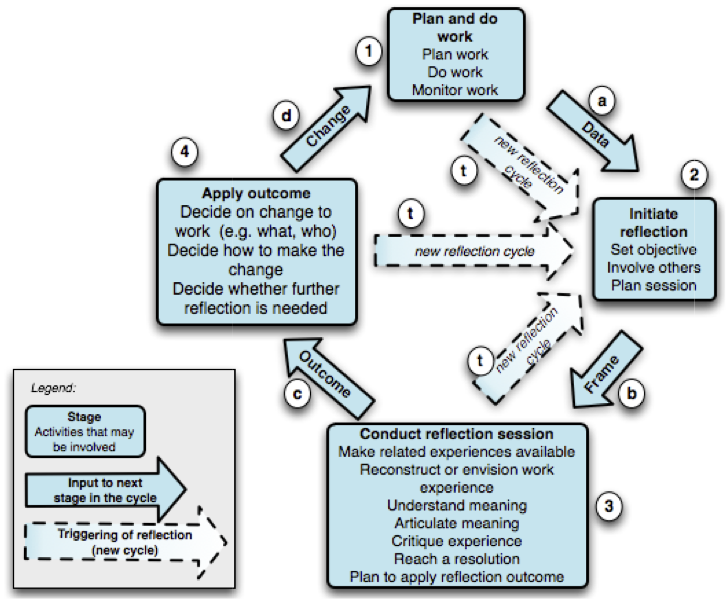
\includegraphics[width=1
	\textwidth]{CSRL} \caption{CSRL reflection cycle. Figure adapted from \protect\autocite{Krogstie:2013kf}} \label{fig:csrl-model} 
\end{figure}

Figure \ref{fig:csrl-model} depicts the models in terms of \emph{stages}, \emph{inputs} and \emph{triggers}. A \emph{stage} includes sub-activities that can be supported with technology, \emph{inputs} are either raw or more or less contextualised data being exchanged among stages; \emph{triggers} are either external events or internal mental processes that initiate a reflection session. Reflection can be triggered during work, while a change is about to be applied, or during the reflection session itself. In general, reflection seems to be triggered by awareness of discrepancy between expectations and the current experience.

Triggers also allow for including more actors in the reflection process, iteratively starting a new cycle based on the results of previous ones. For instance, the outcome of a personal consideration (e.g.~how a crisis procedure is applied) might be brought in a team meeting to trigger collaborative reflection, ultimately leading to a change in protocols. In this way, we can look at reflection as a storyline that might involve different actors within the organisation \autocite{PrPK13}.

\section{CSRL applied to crisis training}\label{csrl-applied-to-the-design-of-technology-for-crisis-training}

The CSRL model can be used by designers to choose which technology to use to support reflection activities or do derive requirements for the design of new technologies. For each stage, the CSRL model identifies support that can be provided through technology. For example in the \emph{do work} phase, technology could be used to monitor work and collect data that can be useful for reflection, in \emph{initiate reflection} to set the objectives for reflection or to involve others in the session, in \emph{conduct reflection} to share work experience with colleagues; and in \emph{apply reflection outcomes} to decide how the change to work will be implemented.

The model has driven the development of several software and hardware applications within the MIRROR project; to address reflective learning in the fields of social care, health care, business and emergency aid. For a description of the applications see \autocite{Schwantzer:2014we}. 

In the case of crisis training I identified that the mapping between the activities described by the CSRL model and technology can be placed in three areas (Figure \ref{fig:model-instantiation}):
\begin{itemize}
	\itemsep1pt\parskip0pt\parsep0pt 
	\item technology to \textbf{capture} work experiences (for example by means of automatic sensors, a personal diary application, or a timeline visualisation) 
	\item technology to \textbf{re-create} work experiences, making use of the captured data to trigger and assist a reflection session with relevant information (for example by allowing to re-evaluate a past experience from multiple point of views, in a context that help making sense processes during debriefing) 
	\item technology to \textbf{generate} new, realistic work experiences for training purposes (for example via virtual worlds, serious games, or tabletop exercises) 
\end{itemize}

The mapping has been derived by the field studies performed and it has not yet included the stages of \emph{initiate reflection} and \emph{apply outcomes}.

\begin{figure}
	[htb] \centering 
	\includegraphics[width=1
	\textwidth]{model-instantiation} \caption{Instantiation of the CSRL model to support crisis training} \label{fig:model-instantiation} 
\end{figure}

The three areas have the common need for innovative interfaces between people and technology. Yet the design of such user interfaces aims at different goals. During \emph{capturing} the interface should allow the capture of a variety of quantitative data and user-submitted information without interrupting crisis work. The stage of \emph{re-creating} experiences need tools for data visualisation and manipulation capable to re-create a work experiences in a context that promote reflection. Finally \emph{generating} experiences needs interfaces to bring realism and engagement of real crises into a simulated environment. Notably, the \emph{capture} of experiences is done during the work, which is subject to strict protocols that limit the design space for the technology.

In the following chapter I will investigate how recent advances in the field of sensing-based interaction can provide theoretical tools from human-computer interaction theory for the design of user interfaces for capturing, re-creating and generating crisis work experience. 

\chapter[Theoretical underpinning:\\Sensing-based interaction][Sensing-based interaction]{Theoretical underpinning: Sensing-based interaction}\label{interaction}

This chapter reviews theories in Human-Computer Interaction (HCI) to inform the design of computer interfaces to support the \emph{capture}, \emph{re-create} and \emph{generate} crisis training experience.

Field studies conducted by the author during physical simulations of crisis work (a description is available in Chapter \ref{research}) have identified requirements for the design of technologies to support the CSRL activities. To support the \emph{capture} stage the design goal emerged is to provide unobtrusive, distraction-free user interfaces to enable and control data collection. During \emph{re-creation} and \emph{generation} stages the objective is to provide situated, highly interactive user experiences using data to promote reflection.

The intrinsic physicality of crisis work was very visible during field studies. When I started to design computer interfaces to support reflection for this very specific target group, it seemed to me advantageous to preserve some extent of \emph{physicality} into their user-experience with technology. After surveying HCI literature for theoretical frameworks to facilitate integrating \emph{physicality} into computer interfaces I focused on the aspects of \emph{embodiment} and \emph{tangibility}. Those are characterising traits of sensing-based interfaces \autocite{Benford:2005bo}.

Sensing-based interfaces is rather a broad term referring to user interfaces that rely on sensor technology to make interaction between people and computers more intuitive and effective \autocite{Zhai:2005jm}. They allow for post-\emph{WIMP} \autocite{VanDam:1997tz} interaction paradigms, to design user interfaces not relying on traditional \emph{W}indows, \emph{I}cons, \emph{M}ouse and \emph{P}ointers metaphors. Instead, sensing-based interfaces promote ``embodied interaction, tangible manipulation, physical representation of data and embeddedness in the real space'' \autocite{Hornecker:2006uq}. According to Rogers and Muller \autocite*{Rogers:2006te} sensing-based interaction allows the design of systems capable to deliver relevant information at appropriate times, which is critical to trigger and sustain reflection; and enable ``hands-free control'', which is fundamental for unobtrusively capturing data in action.

Theoretical tools to include \emph{embodiment} and \emph{tangibility} into user interfaces are reviewed in the next sections.

\section{Tangible and embodied interaction}\label{tangible-interfaces-and-embodied-interaction}

Embodied interaction, as defined by Dourish \autocite{Dourish:2001vc}, is a collection of trends emerged in HCI, relying on the common ground to provide a more natural user interaction with digital information. Embodied interaction makes an enormous shift from previous paradigms. Moving from time to space, it takes the interaction ``off the screen'' into the real world \autocite{Dourish:2001vc}; distributing inputs in space, de-sequentialising interaction and reducing the gap between where the information is created where it is accessed. The interactional media, with its affordances, is the interface: ``By treating the body of the device as part of the user interface --an embodied user interface-- we can go beyond the manipulation of a GUI (Graphical User Interface) and allow the user to really directly manipulate an integrated physical-virtual device'' \autocite{Fishkin:2000df}

Tangible user interfaces (TUIs) are computer interfaces in which technology is embedded into physical objects and spaces, enabling an \emph{embodied} interaction with digital information. In this picture, unlike GUIs which manipulate virtual elements (e.g.~icons) with the aid of keyboard and mouse, TUIs integrate both representation and control of computation into physical artefacts \autocite{krumm2009ubiquitous}. This approach allows system designers to be free to experiment with new type of metaphors, taking advantage of users' physical skills and providing interfaces which exploit people's knowledge with the everyday, non-digital, world \autocite{Jacob:2008vm}. Since the ways the manipulation of physical media profoundly differs from the manipulation of the digital \autocite{Terrenghi:2007uv}, metaphors adopted for the digital world need to be redesigned to meet physical affordances. The design of TUIs as well as other sensing-based interfaces poses new challenges to designers \autocite{Bellotti:2002wg}. Those challenges were also further elaborated by Marquardt and Greenberg \autocite*{Marquardt:2012tg}. Several terms have been used to characterise systems of tangible interfaces: e.g. \emph{tangibles}, \emph{graspables}, \emph{tokens}, \emph{containers}, \emph{phicons}, \emph{tangible bits}; in the following I will call them \emph{tangibles}.

\emph{Tangibles} are part of the broad field known as Ubiquitous Computing, widely attributed to the work of Mark Weiser. In his pioneering article on Scientific American \autocite{weiser1991computer} he envisioned a close coupling between the digital and the physical, to the extent that the technology ``disappears into the fabric of the everyday life''.

\subsection{Theoretical frameworks}\label{frameworks}

Over the years several research initiatives have proposed frameworks either to characterise systems of tangibles, e.g. \autocites{Fishkin:2004uv}{Jacob:2008vm}{Hornecker:2006uq}; or to provide opportunities and guidelines to support the design of new TUIs, e.g. \autocites{Benford:2005bo}{Shaer:2004ta}{Rogers:2006te}.

In 2000, Ullmer and Ishii \autocite*{Ullmer:2000vf} took the first steps investigating the design of tangibles. They defined TUIs as computer interfaces that give physical form to digital information, rethinking the interfaces itself as being composed by some sort of ``tangible bits'' \autocite{Ishii:1997ur}. In order to help understanding and building tangibles, they created a conceptual framework and interaction model called MCRit. MCRit, an abbreviation for Model-Control-Representation (tangible and intangible), adapts the Model-View-Controller (MVC) model of GUI-based interaction to the design of tangibles. Besides MCRit highlights the ``seamless integration of control and representation'' characteristic of tangibles, it redefines the capability of the interface to provide information as a balance between its physical representation (the object's shape and affordances) and a intangible one (e.g.~computer graphics and sounds) (Figure \ref{fig:mcrit-model}). For example by augmenting physical objects with video-projections and sounds in order to extend the static representation of an object with an intangible, dynamic one.

\begin{figure}
	[tbh] \centering 
	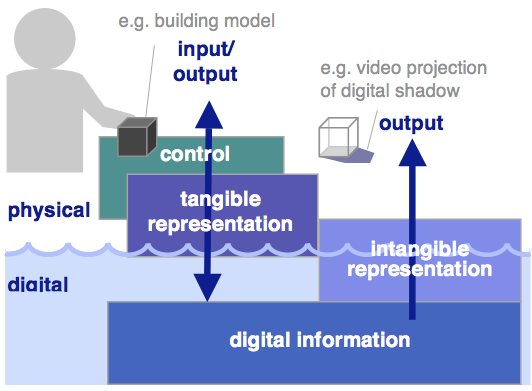
\includegraphics[width=0.6
	\textwidth]{mcrit} \caption{Tangible and intangible representations of TUI. Figure adapted from \protect\autocite{Ishii:2008fh}} \label{fig:mcrit-model} 
\end{figure}

In fact one of the main pitfalls of TUIs is that while GUIs serve as generic purpose interfaces by allowing multiple kinds of tasks, defined by the software; TUIs serve as special purpose interfaces, each one tailored to a specific set of actions (defined by physical affordances and constrains). A tangible interface can hardly be adapted to work in a context that differs from the one it has been designed for. This trade-off has been defined by Jacob \autocite*{Jacob:2008vm} between Reality and Versatility: it trades the capability of a system of doing many different tasks (like browsing photos, writing a document) with the possibility to accomplish only one single task with a higher level of realism or simplicity.

Following the work of Ullmer and Ishii other research has looked at tangibles from other perspectives. Jacob et al. \autocite*{Jacob:2008vm} identifies four interaction themes with the real world that can be leveraged for the design of TUIs. Hornecker and Buur \autocite*{Hornecker:2006uq} present four topics to be considered in scenarios where tangible interaction has social aspects. Fishkin \autocite{Fishkin:2004uv} presents an aggregated perspective on other frameworks, categorising tangible systems as a continuum spectrum according to the level of embodiment and metaphor they provide. Finally Ullmer et al. \autocite{Ullmer:2005jz} envision TUIs as a systems of \emph{tokens} and \emph{constraints}. The former are discrete physical objects that represent digital information, the latter mechanical or visual confining regions that are mapped to digital operations. By the interaction phases of association and manipulation of tokens within a system of constraints it is possible to map physical actions to a set of computational operations in a grammar of ways. For example the presence or absence of a token in a constrained area could be easily digitalised in binary information to trigger a digital operation. For a literature review on other frameworks see \autocite{Mazalek:2009uy} and \autocite{Shaer:2009fx}.

\subsection{Applications in reflective learning}\label{applications-of-tangibles-in-reflective-learning}

Although the relation between tangibles and reflection has not been thoroughly investigated, several works have shown that TUIs might be beneficial for learning \autocite{Marshall:2007dr}; for a review see \autocite{omalley:hal-00190328}. Although these often focus on applications of TUIs for children and classroom environments, TUIs might have possible benefits on learning on a broader scope. Those benefits include the support to more natural \autocite{Terrenghi:2005gq} and situated \autocite{Klemmer:2006ez} learning, and increased reflection and engagement \autocite{Rogers:2006te} due to the link between physical action and digital feedbacks. Moreover TUIs foster collaboration \autocite{Rogers:2003tt}, in which they increase visibility of others' actions and allow for concurrent interaction.

Theoretical tools adapted from the presented frameworks have driven the design of sensing-based interfaces described in Chapter \ref{results}.

In the next chapter I will present the research methodology adopted throughout the work, providing details on the field studies performed and prototypes built. 

\chapter{Research methodology}\label{research}

\todo[inline]{Revision5}

The aim of this chapter is to present the research methods and tools adopted. Although not all of these methods have been explicitly reported in the papers, they have been important to understand the users and the domain.

\section{Research overview}\label{research-overview}

The work in this thesis is based on design science research \autocites{Hevner:2010gc}{March:1995gm}. Design science provides theoretical tools to study and understand a specific domain, as well as processes to build artefacts with the aim at improving an environment \autocite{simon1996sciences}. The work unfolded by interweaving field studies to understand the crisis domain, and turn opportunities observed into system requirements; with design iterations to build technologies to address those opportunities. 

The design science approach meets the aim of this research work, which lies in the design of technologies for better crisis training (RQ1-RQ2). The focus of design science on rapid iterations between the construction of artefacts and their evaluation \autocite{Hevner:2010gc} also makes a good strategy for the investigation of RQ3.

Hevner et al. \autocite*{Havner2004} describes design research as a sequence of three tightly coupled cycles of activities (Figure \ref{fig:design-cycles}). Each of the three cycles must be present and visible in a design science research project \autocite{Hevner:2010gc}.
\begin{figure}
	[tbh] \centering 
	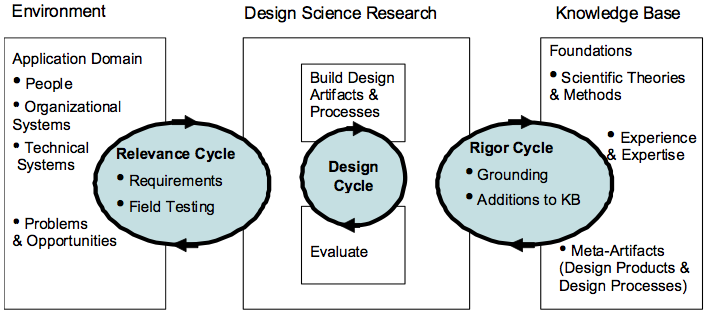
\includegraphics[width=1
	\textwidth]{design_cycles} \caption{The design cycles, figure adapted from \protect\autocite{hevner2007three}} \label{fig:design-cycles} 
\end{figure}
\begin{itemize}
	\item The \emph{relevance cycle} involves designing and running field studies with exploratory or evaluation purposes. While the former type derives requirements for technology to be implemented in prototypes, the latter type cycles between defining acceptance criteria and introducing technologies into the environment for field testing, aiming at improving artefacts until research goals are met. 
	\item The \emph{rigor cycle} includes both a continuous process of keeping design work informed by relevant grounding theories, and a retrospective effort in validation and extension of those theories. This cycle qualifies the research to maintain an innovation approach able to bring research contributions. 
	\item The \emph{design cycle} rapidly iterates between the production of a prototype and its formative evaluation to gather feedback and refine the design. This stage is fed with requirements from the relevance cycle and theories from the rigor cycle; it returns artefacts for field test to the former and theoretical knowledge to the latter. 
\end{itemize}

To implement the main research strategy, several methods have been adopted. I used a mix of qualitative research methods to account for the unpredictability in an in situ study \autocite{Rogers:2007gv}. Observations, interviews and researchers' notes were the primary means to collect data on the field. Scenarios and personas drove the design phase. Open source hardware and software toolkits were largely adopted to turn mockups into working prototypes. Finally questionnaires and interviews were used during prototypes formative evaluations and field tests.

The choice of these methods required to have access to people, knowledge and protocols of organisations working in the crisis domain. This research strategy was facilitated by having crisis training organisations, as members of the MIRROR consortium. Moreover, throughout the duration of the work, discussions with members of the consortium and co-authored publications helped in shaping research strategies and partially influenced the work.

\section{Research activities}\label{research-activities}

This section details the activities performed and how methods have been instantiated. A chronological account of the research process is provided in Figure \ref{fig:research-activities}.
\begin{figure}
	[ptb] \centering 
	\includegraphics[width=1
	\textwidth]{timeline} \caption{Timeline of research activities} \label{fig:research-activities} 
\end{figure}

During the progress of the research, several activities concurrently unfolded intra and inter the \emph{relevance}, \emph{design} and \emph{rigor} cycles.

The work started off with two exploratory field studies aimed at understanding the crisis training domain, its needs and challenges. Soon enough early design ideas were turned into low-to-high fidelity prototypes in short iterations. 

In the central course of research, activities iterated between new prototype releases and consequent formative evaluations; often recurring to new field studies to keep the design process updated with new requirements. Prototypes presented in focus groups with workers facilitated discussions, triggering a better understanding of the domain, which in turn led to new ideas. Furthermore, prototypes facilitated the reminiscence of work experience, bringing new perspectives into the study.

In the final iterations of the work, working prototypes acted as means to validate and extend theories as part of the \emph{rigor cycle}. Results from evaluations provided insights to validate and extend theories of reflective learning, as reported in P6. 

Research outcomes were reported in academic publications (Chapter \ref{results}) and research contributions (Chapter \ref{contributions}) emerged. Finally the work focused on exploring generalisation during research abroad (Appendix \ref{abroad}) and on investigating commercial exploitation of research contributions (Section \ref{exploitation-of-research-contributions}).

Throughout the process literature in reflective learning (Chapter \ref{csrl}) and sensing-based interaction (Chapter \ref{interaction}) informed the design work. While the former identified \emph{what} activities and processes to trigger reflection can be enhanced with technology; the latter provided guidelines on \emph{how} to design technology artefacts.

In the following sections, a description of field studies performed and methods adopted are provided in Section \ref{field-studies}. The production and formative evaluation of prototypes is covered in Section \ref{prototypes}.

\subsection{Field studies}\label{field-studies}

The primary investigation method selected to understand the crisis domain and evaluate artefacts produced by the design cycle has been \emph{field studies} \autocite{robson1993real}. In this work, field studies had a twofold objective. Some studies acted as exploratory research to inform the design of technology, some others as field evaluation for the tools developed; some else covered both aims.

An overview of the field studies performed between years 2011-2014, in relation with research questions and papers, is presented in Table \ref{tab:field-studies}

\begin{table}
	[h] \centering \caption{List of field studies performed} \label{tab:field-studies} 
	\begin{tabular}
		{@{}lllllllll@{}} 		%\begin{tabular}{@{}p{0.3cm}p{3cm}p{0.3cm}p{0.3cm}p{3cm}p{0.25cm}p{0.25cm}p{0.25cm}p{1.5cm}}
		\toprule & & \multicolumn{2}{c}{Aim} & & \multicolumn{3}{c}{Methods} & \\
		\cline{3-4} \cline{6-8} \noalign{\smallskip} ID & \specialcell[b]{Date,\\duration} & 
		\begin{turn}
			{90}Exploratory
		\end{turn}
		& 
		\begin{turn}
			{90}Evaluation
		\end{turn}
		& Participants & 
		\begin{turn}
			{90}Observations
		\end{turn}
		& 
		\begin{turn}
			{90}Interviews
		\end{turn}
		& 
		\begin{turn}
			{90}Questionnaires
		\end{turn}
		& Papers \\
		\midrule \noalign{\smallskip} F1 & \specialcell[t]{Mar. 2011,\\2 days} & \textbullet & & several teams & \textbullet & \textbullet & & P1 \\
		F2 & \specialcell[t]{Oct. 2011,\\3 days} & \textbullet & & \specialcell[t]{several teams,\\1 manager} & \textbullet & \textbullet & & P1, P3 \\
		F3 & \specialcell[t]{Oct. 2012,\\2 days} & \textbullet & \textbullet & \specialcell[t]{5 field workers,\\1 manager} & \textbullet & \textbullet & & P1, P3 \\
		F4 & \specialcell[t]{Apr. 2013,\\3 days} & \textbullet & \textbullet & \specialcell[t]{4 field workers,\\1 manager} & \textbullet & \textbullet & \textbullet & P1, P3, P2 \\
		F5* & \specialcell[t]{Dec. 2013,\\30 days} & & \textbullet & 8 field workers & & & \textbullet & P2, P3, P6 \\
		F6 & \specialcell[t]{Apr. 2014,\\2 days} & & \textbullet & \specialcell[t]{27 field workers,\\1 manager} & \textbullet & & \textbullet & P2, P3, P6 \\
		\noalign{\smallskip} \hline \noalign{\smallskip} \multicolumn{9}{l}{\small{*The author was not present during the study}} \\
		\bottomrule 
	\end{tabular}
\end{table}

The setting for the majority of the studies was medium to large-scale physical simulation of crisis work (drills). The first exploratory study (F1 in Table \ref{field-studies}) took place during attendance at a real crisis management event. A description of a typical physical simulation was provided in Chapter \ref{crisis}.  Objectives of those simulations were to train workers against protocols, rescue procedures, and test of equipment. Notably, the observed events also offered opportunities for team building and sharing of experiences, as part of official and unofficial social gatherings.

The observed training events, involved personnel from a range of crisis management organisations operating in northern Italy, coordinated by \emph{ANPAS-Piemonte}\footnote{ANPAS-Piemonte crisis management organisation - http://anpas.piemonte.it} and \emph{SEIRS}\footnote{SEIRS crisis management organisation - http://seirs.org} organisations. Contacts with these institutions have been initiated via a partner of the MIRROR consortium. A wide range of roles were observed, including field workers (firefighters, paramedics, police agents), team coordinators, disaster manager, technical and radio staff. The number of participants in our studies varied between dozens of workers observed in the exploratory studies to smaller groups who where actively involved during interviews and prototype evaluations.

Observations, researcher notes and interviews were the primary means to collect data. In addition questionnaires were employed during evaluation studies.

Workers were shadowed while performing rescue work. To this respect, my role as observer strived to be, as defined by Walsham \autocite*{Walsham:2006bo}, \emph{neutral}; meaning that people being shadowed should not perceive the researcher as biased by previous views on people, processes or organisations. Video recording, performed with both handheld and head-mounted cameras worn by simulations' participants, provided multiple point of views on the observed events. Qualitative data collection methods were supplemented by descriptions of protocols, procedures and best practices provided by the organisations involved in the studies. Data captured were handled in observance of NTNU and MIRROR policies. No compensation was given to the workers after participation to the studies.

Data collected from researchers' notes, interviews and questionnaires, together with video recording and logs were analysed with qualitative research methods \autocite{robson1993real}. The focus of the analysis was twofold.

During exploratory studies the focus of attention was on how practitioners capture aspects of their work experiences. It allowed to identify on one hand what information is relevant for reflection; on the other hand what technology to capture information is already in use or is desired. The outcome of this phase produced a set of requirements to drive the design of technology; including challenges, system requirements, scenarios and personas. This result fed the \emph{design cycles}, for the construction of prototypes.

During evaluation studies the focus was on measuring how well prototypes perform against user acceptance, usability of the systems, and impact on learning. Selected workers were provided with prototypes for test during field work. Workers were walked through the use of technology by a researcher and a set of tasks to be accomplished was given to each participant. Participants' interactions with the technology were observed and video recorded with wearable cameras; in addition prototypes were configured to log modes of operation.

After each test, researchers followed up with observations, interviews and questionnaires. Questionnaires offered a high-level quantification of feedback, while observations and interviews aimed to ground this feedback in the context of usage. Questionnaires in use during the evaluations were adapted from the MIRROR evaluation toolbox \autocite{Knipfer:2012vi}, which provides surveys to measure user acceptance, perceived learning success, and the intention to change behaviour. These questionnaires are a generic instrument that build on the Kirkpatrick framework \autocite{kirkpatrick2009evaluating}. 

\subsection{Design iterations}\label{prototypes}

Design and prototyping work was driven by requirements, scenarios and personas generated during field studies. The design process followed a \emph{user centred approach} \autocites{MAGUIRE:2001dp}{Gulliksen:2003hd}.

A total of eight prototype iterations were completed. Table \ref{tab:prototypes} overviews the prototypes developed, tools and technologies used during development in relation with the papers that described the work. Prototypes included a mobile app (\emph{CroMAR}, two iterations), wearable sensors (\emph{WATCHiT}, four iterations) and a technology-augmented board game (\emph{Don't Panic}, two iterations). 

\begin{table}
	[!p] \centering \caption{List of prototypes built} \label{tab:prototypes} 
	\begin{threeparttable}
		\begin{tabular}{@{}llllllll@{}} 
			\toprule 
			& & & & \multicolumn{3}{l}{Development}  \\
			\cline{5-7} \noalign{\smallskip} 
			\specialcell[b]{ID\\Ver.} & Name & Released & Prototyping tools & 
			\begin{turn}
				{90}Software
			\end{turn}
			& 
			\begin{turn}
				{90}Hardware
			\end{turn}
			& 
			\begin{turn}
				{90}Material
			\end{turn}
			& Papers \\
			\midrule \noalign{\smallskip} C1 & CroMAR & Jul-11 & iOS, & \textbullet & & & P1,P2 \\
			C2 & & Jul-12 & Augmented Reality & \textbullet & & & P2 \\
			\hline \noalign{\smallskip} W1 & WATCHiT & Jan-12 & Arduino, Textiles & \textbullet & \textbullet & & P3 \\
			W2 & & Aug-12 & ZigBee, Bluetooth & \textbullet & \textbullet & & P3 \\
			W3 & & Sep-12 & & \textbullet & \textbullet & & P3 \\
			W4 & & Aug-13 & & \textbullet & \textbullet & \textbullet & P2, P3 \\
			\hline \noalign{\smallskip} D1 & Don't Panic & Mar-13 & Paper, wood & & & \textbullet & P4, P5 \\
			D2 & & Aug-13 & \specialcell[t]{Sifteo, RapsberryPi\\Laser cut} & \textbullet & \textbullet & \textbullet & P5 \\
			\bottomrule 
		\end{tabular}
		\begin{tablenotes}
			\item 
			\includegraphics[width=\linewidth]{prototypes} 
		\end{tablenotes}
	\end{threeparttable}
\end{table}

Building each prototype involved a mix of software, hardware and material development. Software was written for a variety of systems. The development of hardware included design, production and test of electronic circuits. In some prototypes the circuits developed were embedded in hard-shells that were custom-designed and produced in plastic or wood (material development). The design of the appearance for the resulting software/hardware hybrid artefact aimed either at protecting electronic circuits during field test or to provide specific affordances for interaction.

During development I largely adopted rapid prototyping techniques in order to keep design iterations short and produce incremental improvements based on frequent feedbacks exchange with end users. To this end a wide range of open source toolkit were used, including Arduino\footnote{Arduino platform - \url{http://arduino.cc}} and RaspberryPi\footnote{RaspberryPi platform - \url{http://raspberrypi.org}} hardware development platforms. Digital manufacturing techniques were largely adopted, including CAD software, 3D printing and laser-cut production. These activities were essential to the development of knowledge to the investigation of RQ3. 

After each prototype was built, a formative evaluation followed. User testing allowed for maintaining a user-centred design perspective, to introduce new ideas into the process, and to test prototypes in a controlled setting before releasing them for field testing.

\begin{table}
	[h] \centering \caption{List of focus groups performed} \label{labtests} 
	\begin{tabular}
		{@{}lllllllll@{}} \toprule 
		ID & Date & Participants & Prototypes tested \\
		\midrule 
		G1 & Apr-12 & 9 field workers & W1, D1 \\
		G2 & May-12 & 1 disaster manager & C1, W1 \\
		G3 & Jul-13 & 3 field workers, 1 manager & D2 \\
		G4 & Sept-13 & 8 IT students, 4 HCI experts & D2 \\
		\bottomrule 
	\end{tabular}
\end{table}

To this intent, focus groups with crisis workers were performed. A list of focus groups performed, and prototypes tested is depicted in Table \ref{labtests}. Focus groups with workers were essential for fuelling the design activity. Moreover, meetings often saw the participation of the same workers who were previously shadowed during physical simulations. It was therefore possible to ground discussions into specific episodes previously observed on the field.

\begin{figure}
	[tbh] \centering 
	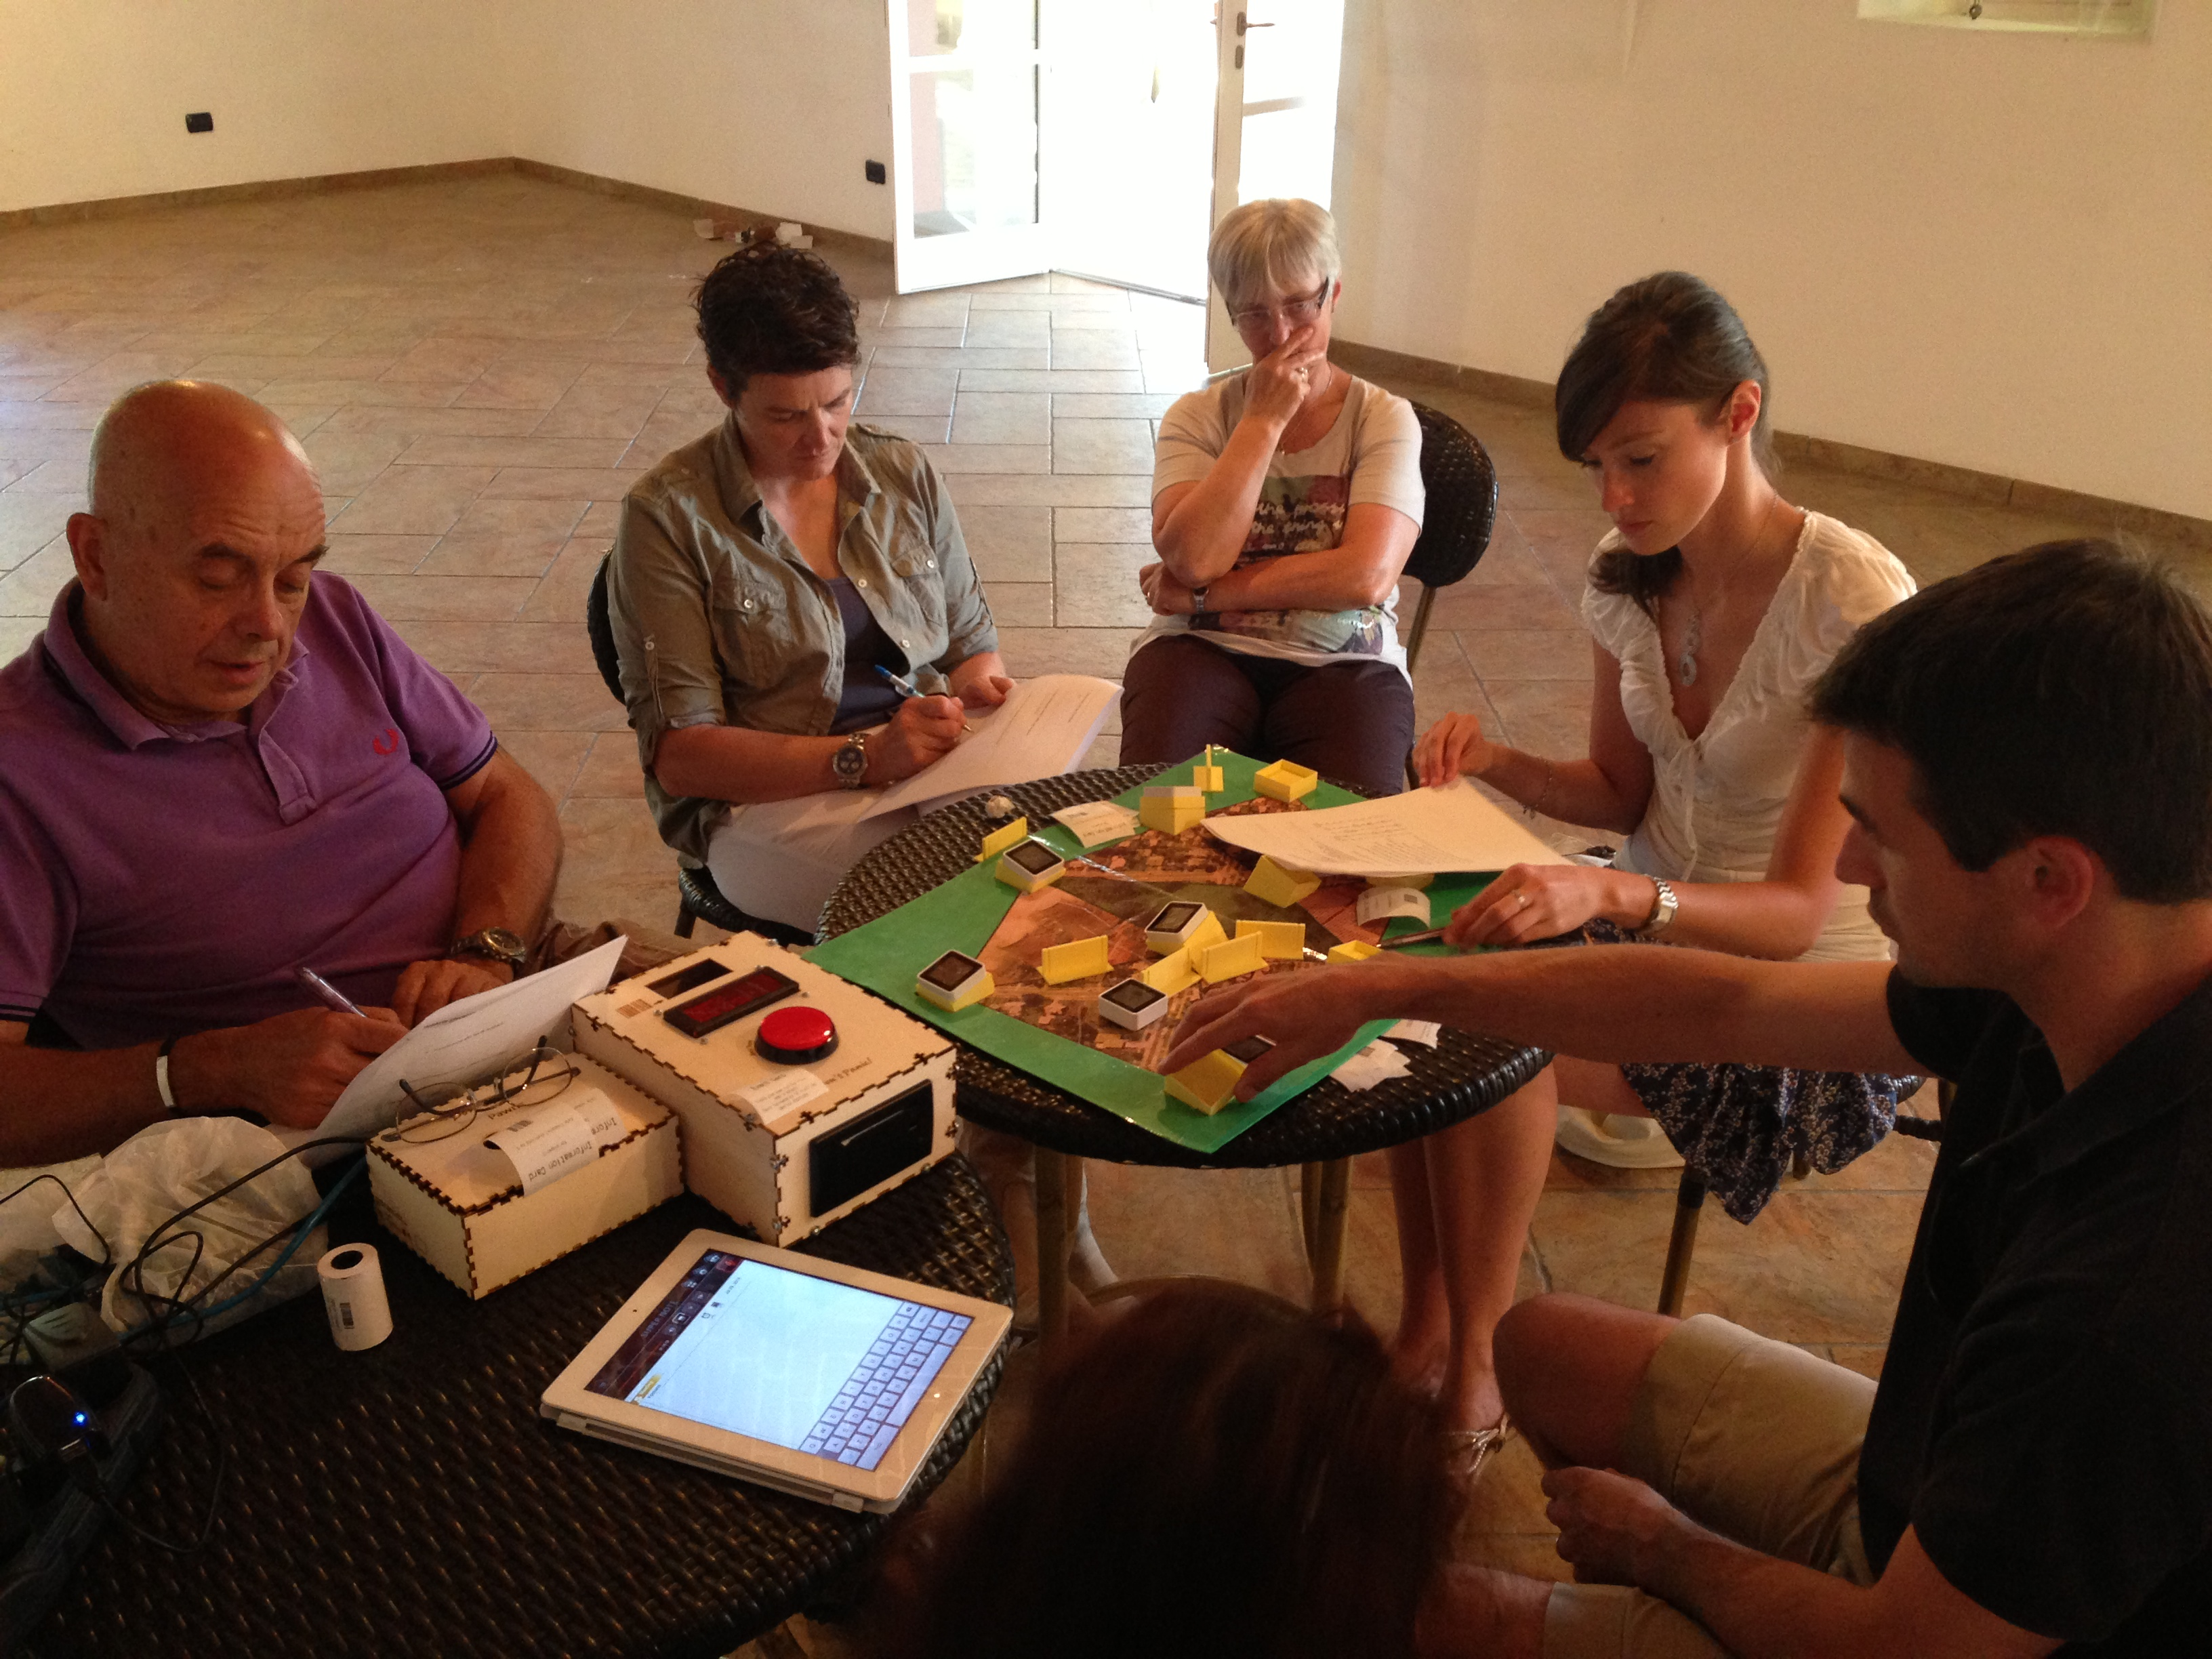
\includegraphics[width=1
	\textwidth]{d2_prototype} \caption{Participants of the G3 group filling in SUS questionnaires, after the test of D2 prototype} \label{fig:focus-group} 
\end{figure}

During focus groups low and high fidelity prototypes were evaluated. The typical setting of focus groups performed is represented in Figure \ref{fig:focus-group}. Low-fidelity prototypes acted as technology probes \autocite{Hutchinson:2003il}. Despite their evident usability issues, they were essential to create new scenarios of use and identify technological and usage challenges. Higher-fidelity prototypes underwent usability tests \autocite{Dumas:2009th} using System Usability Scale (SUS) \autocite[page 189]{jordan1996usability}.

In the following chapters the papers that added up to the results of this thesis are presented.
\chapter{Results}\label{results}

\todo[inline]{Revision 3}

In the previous chapter the research background and methodology adopted during the work were presented. This chapter summarises the papers that added to the research contributions.

\section{Papers}\label{papers}

The research work has been published in two journal papers and four conference papers, one paper is currently ready for submission. In this section, papers that presents the results of this thesis are summarised. Each summary includes: 
\begin{itemize}
	\itemsep1pt\parskip0pt\parsep0pt 
	\item Title 
	\item Authors and roles in the paper 
	\item Abstract of the paper
	\item Where the paper was published 
	\item A short description of the results 
	\item The paper's relation to research questions 
\end{itemize}

Papers are reprinted in full in Appendix \ref{papers} of the thesis.

In addition to the papers presented in this section this PhD work has produced fourteen peer-reviewed secondary papers presented in conferences and workshops which are omitted in this section. Those works present incremental achievements in research that led to the results presented here. A brief description of secondary papers is included in Appendix \ref{secondary-papers}

\section[CroMAR: Mobile Augmented Reality for Supporting Reflection on Crowd Management]{Paper 1} \label{paper-1}

\emph{Title}: CroMAR: Mobile Augmented Reality for Supporting Reflection on Crowd Management

\emph{Authors}: Simone Mora, Alessandro Boron and Monica Divitini

\emph{Authors' contributions}: Mora led the research and the paper writing. He was actively involved in design, development, and evaluation of the system. Boron developed part of the described prototype and contributed to the paper with the description of the technical implementation. Divitini provided~general~supervision for the research and the paper writing. 
\begin{quote}
	\emph{Abstract:} This paper discusses the usage of Mobile Augmented Reality (MAR) to support reflection on past events, using reflection on crowd management as scenario. Computer based support to reflection generally relies on the visualization of information connected to the experience one is reflecting upon. Different metaphors have been adopted to support easy access to relevant information within the reflection process, e.g., timelines and word clouds. In this context, MAR represents an interesting alternative because it can be used to promote reflection in the specific location of the event by augmenting it with relevant information. In this way, the authors can expect the reflection process to be grounded in a context that helps to make sense of the information and reflect on alternative paths of action. The paper presents the scenario of usage, together with the design, development, and evaluation of the prototype, CroMAR. Based on this experience, the authors identify challenges connected to the usage of Mobile Augmented Reality in terms of support for reflection, interaction, and design methodology. 
\end{quote}

\emph{Published in}: International Journal of Mobile Human Computer Interaction (IJMHCI), 2012

\emph{Description}: This paper investigates the adoption of Mobile Augmented Reality (MAR for short) to support debriefing of work practices that rely on management of resources in space. To date, it is the first time that MAR is used for such purpose. Crowd management, an activity typically performed by civil protection organisations during large public events, is scrutinised to investigate the use of augmented reality to support (collaborative) reflection processes after the event is concluded. Crowd management is a critical activity both for crisis preparedness and during crisis management.

CroMAR, an iPad app designed by the authors, demonstrated the use of MAR for reflection. The system developed focuses on supporting navigation of reflection-useful information along the time and space dimension. Visualisation of information is provided in-situ, in a physical context that helps making sense of the information and reflect on alternative paths of actions. Also, the system provides support in involving others in the reflection process and in sharing of its outcome.

The proposed design has been implemented in a working prototype of an iPad app (Figure \ref{fig:cromar-prototype}), with focus on modularity and extensibility. The prototype has been evaluated in a focus group with experts. The study highlights challenges in supporting reflective learning with MAR tools, with focus on user experience. First the research requires a better understanding of the conditions that makes MAR a better approach compared to other visualisation approaches (e.g.~maps, timelines). Second, it claims the need for providing scaffolding mechanisms to the reflection process; to make sure that relevant information for a given session is explored. Acknowledged by experts that the physical exploration of space provide scaffolding for exploration of information, it is necessary to study when it actually promotes reflection. 

\begin{figure}
	[tbh] \centering 
	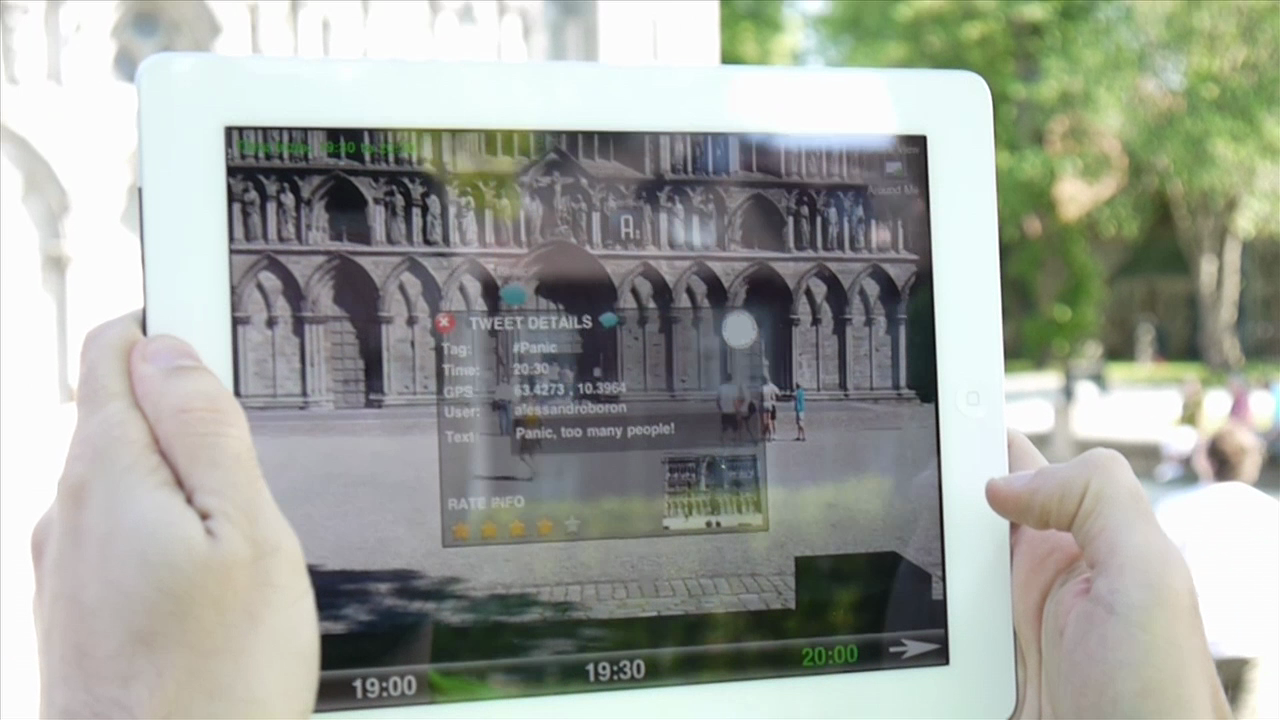
\includegraphics[width=1 
	\textwidth]{cromar_1stproto} \caption{CroMAR early prototype} \label{fig:cromar-prototype} 
\end{figure}

During our evaluation, the overall user experience with the prototype was hampered by lack of functionalities and lack of suitable hardware platforms. The experience is disrupted by the lack of tools for filtering the data visualised, to remove redundant information and prioritise the important ones. On the other side, the choice of iPads 2 has limitation due to device weight and size which can only be comfortably hold by the user for a few minutes.

The results from this paper have fed new design iterations for CroMAR. The design of new functionalities has followed more closely the guidelines provided by the CSRL model that was being developed at the time. Meanwhile lighter and smaller version of the iPad came to the market which allowed an extended use for our system. A new prototype of CroMAR and its closer mapping to the CSRL model is described in P2.

\emph{Relation to the research questions: } The paper started the investigation of RQ2, ``\RQii'' 

\section[Supporting Debriefing with Sensor Data: A Reflective Approach to Crisis Training]{Paper 2}\label{paper-2}

\emph{Title:} Supporting Debriefing with Sensor Data: A Reflective Approach to Crisis Training

\emph{Authors:} Simone Mora and Monica Divitini

\emph{Authors' contributions:} Mora led the research and the paper writing. He also led the design of the presented technology and directly implemented or supervised the implementation of the prototypes. Both authors attended the evaluation studies. Divitini provided general supervision for the research and the paper writing.

\begin{quote}
	\emph{Abstract:} In this paper we present our exploration into the use of sensor data to promote debriefing after training events simulating work experiences. In this way we address one of the core challenges of crisis training, namely the difficulty to exploit the full potential of training events, e.g.~during drills. The paper is theoretically grounded in the theory of reflective learning. The theoretical understanding is used for informing the design of WATCHiT, a wearable device for collecting sensor data during an event, and two applications for promoting debriefing in two different scenarios, CroMAR and Procedure Trainer. CroMAR supports disaster managers during in-situ debriefing after large events, while Procedure Trainer supports a team in reflecting after the simulation of a medical emergency procedure. The evaluation of the two applications shows that sensor data can be successfully used to support debriefing in both scenarios. Based on our experience, we draw lessons learned for the design of systems supporting debriefing in training events. 
\end{quote}

\emph{Published in:} Proceedings of Information Systems for Crisis Response and Management in Mediterranean Countries (ISCRAM-MED), 2014

\emph{Description:} The paper focuses on supporting with sensor data the activity of debriefing after training events simulating work experiences (e.g.~physical simulations). 

To increase the efficacy of debriefing, and thus their impact on crisis preparedness, it is important to exploit the full potential of training events, which are costly to organise. There are different forms of debriefing, all complex activities that may vary in terms of details and people involved according with the emergency scenario workers have been training on. Debriefing is made difficult by the highly distributed nature of the work, the co-existence of different partial experiences and lack of data to complement human memories of the event. The paper addresses those challenges presenting an ecology of three applications of sensing-based technology to assist different debriefing scenarios. Two applications: \emph{CroMAR} and \emph{WATCHiT} have been described in P1 and P3 and are here presented in the last stage of their evolution. Trainer, introduced in this paper, is an smartphone application to support a quick reflection session on the implementation of protocols (e.g.~medical procedures) that can be done by the worker herself or in a team. In this work technology mapping with the CSRL model is made explicit.

The three applications presented have been evaluated during simulated crisis work events. Building on evaluation results, the paper presets lessons learnt about the use of sensor data for supporting debriefing and the design of systems to support reflection during debriefing. 

\emph{First} it is acknowledged that sensor data has to be complemented by qualitative information in order to set the right focus for reflection and avoid over-sighting qualitative, yet critical aspects of the work that cannot be captured with quantitative methods.

\emph{Second} it suggests the use of \emph{visualisation} and \emph{storytelling} as mechanisms to promote sense-making processes for turning data into useful learning contents. Visualisation helps understanding the data by \emph{re-creating} a context that help spotting discrepancies with other sources and, in turn, to trigger reflection. For this goal it is important that systems allow to compare data against a baseline or other sources. Storytelling happens when a visualisation need to be interpreted and explained both to the self and to others, connecting data to the human memory of the event; as it was observed during evaluations. Also, how to motivate the user in capturing data needed for visualisation and storytelling is still an open challenge.

\emph{Third}, the proposed technologies aim at bringing debriefings out of the traditional office setting but not as substitutes, rather to complement the current practices by creating smooth transitions among different debriefing (and thus reflection) cycles. These propositions will guide future research to leverage sensor data in debriefings.

\emph{Relation to the research questions:} The paper covers aspects of RQ1 ``\RQi'' and RQ2, ``\RQi''

\section[WATCHiT: a modular and wearable tool for data collection in crisis management and training]{Paper 3}\label{paper-3}

\emph{Title:} WATCHiT: a modular and wearable tool for data collection in crisis management and training

\emph{Authors:} Simone Mora and Monica Divitini

\emph{Authors' contributions:} Mora led the research and the paper writing. He also presented the paper at the conference. Mora directly implemented or supervised the implementation of the prototypes. He also conducted the field studies and evaluations. Divitini provided general supervision for the research and the paper writing.

\emph{Published in:} Proceedings of the European Conference in Ambient Intelligence (AMI), 2014 

\begin{quote}
\emph{Abstract:} We present WATCHiT, a prototype of sensor-augmented wristband computer for data collection during crisis response work. During crises, information about the environment (e.g.~to map the territory) and the rescuers (e.g.~for assessment of workers' condition) offers help to support coordination of work, post-emergency debriefing and to build realistic training scenarios. Being each crisis nearly unique it is important to collect data from every single occurrence, yet it is difficult to foresee the type of data and context information that is relevant to capture. WATCHiT features: (1) wearable sensors, (2) easy customisation of the type of information sensed, including both quantitative and qualitative data; (3) an intuitive, distraction-free user interface for controlling the data capturing procedure. Our design process has been driven by user studies during training events characterised by a high degree of realism; our prototype has been successfully evaluated with experts against technology acceptance. 
\end{quote}

\emph{Description:} This paper presents the design research that led the development of WATCHiT, a wearable computer for data collection in-action during crisis response work (Figure \ref{fig:watchit-prototypes}). The design research has followed four steps. Field studies conducted by the authors have produced seven challenges for the design of technology tools to support data collection during real or simulated crisis. Those design opportunities are summarised in Table \ref{tab:design-challenges}. User studies were performed during physical simulation of crisis work. Simulations were organised to provide a high degree of realism, involving dozens of agents; and recreating working conditions as close as possible to real crises.

\begin{table}
	[tbh] \centering \caption{Design challenges for data collection tools in crisis work} \label{tab:design-challenges} 
	\begin{tabular}
		{@{}p{0.05\linewidth}p{0.25\linewidth}p{0.60\linewidth}@{}} \toprule & Challenge & Description \\
		\midrule DC1 & Mobility of work and sensing & It is therefore important to complement data from sensors embedded in the environment with mobile ones. The degree of mobility and thus granularity of data is important. Fine granular data is achieved with sensors worn by first responders. \\
		DC2 & Different crises, different relevant data & Being each crisis almost unique, it is difficult to define which data might be relevant to capture based on generic typologies of crises. \\
		DC3 & Different types of data & Different types of information are relevant to be captured. Including information for assessment of the worker’s safety, for mapping the territory and the work and Information related to the rescued people (e.g. type of injures). \\
		DC4 & Sensor data and user-submitted data & Workers might however provide critical qualitative data that cannot be measured with sensors to complement quantitative ones. \\
		DC5 & Different use, different sharing & While some types of data (e.g. location of agents) can be shared with colleagues to support real-time real time coordination, it's up each agent whether to share or not sensitive data (e.g. stress levels) with peers. \\
		DC6 & Intuitive, hands-free interaction & Workers must focus on the rescue operation and not on data capturing and logging tasks. User interfaces must be very intuitive and distraction-free. \\
		DC7 & Automate and discrete capturing & Capturing data with automatic means doesn't require user intervention but it produce datasets often affected by noise. Discrete capturing requires the user to activate sensors but produces more relevant and contextualised data. \\
		\bottomrule 
	\end{tabular}
\end{table}

The drafted challenges highlight \emph{what} data is relevant to be captured and \emph{how} to collect them. The challenges aim at assisting the design of technology to capture data during crisis work. Data captured can be used to feed reflection during debriefings (as shown in P2) as well as for helping coordination on the field and support decision-making processes.

The challenges drove the design of WATCHiT by establishing three core requirements for the technology. WATCHiT must be implemented to be \emph{wearable} -to achieve the highest degree of mobility in sensing-, \emph{modular} -to allow customisation of the type of data captured to specific crisis scenarios-; finally it has to feature a \emph{distraction-free user interface} to disrupt as little as possible the work. The requirements were gradually implemented in design iterations. Three working prototypes were built (Figure \ref{fig:watchit-prototypes}). Each one featuring a mix of software and hardware technologies, and an increased degree of wearability. Modularity is implemented as an architectural choice with physical sensor modules that allow for transient customisation of sensing capabilities of the device.

\begin{figure}
	[tbh] \centering 
	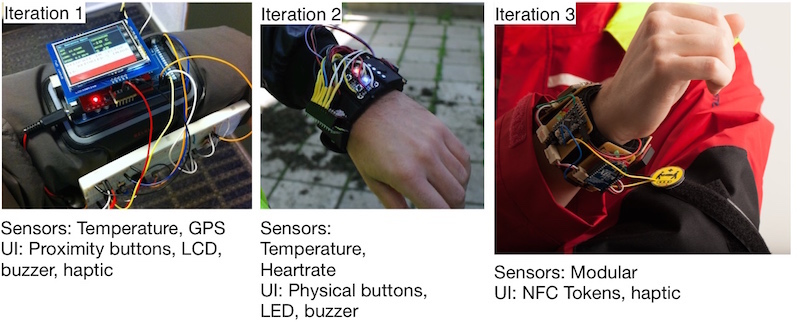
\includegraphics[width=1 
	\textwidth]{watchit_iterations} \caption{Three prototyping iterations for WATCHiT} \label{fig:watchit-prototypes} 
\end{figure}

The requirement for distraction-free user interfaces has been implemented with the design of a novel sensing-based interface grounded on previous works on mnemonic body shortcuts and body-centric interaction \autocites{Guerreiro:2008wt}{Chen:2012wk}. Those works propose to use areas of the body as shortcuts to trigger digital operations in the context to facilitate smartphone-mediated interaction with digital services. In this work body shortcuts are specialised to assist data capturing processes. Areas on work uniforms and tools (identified by RFID tags) trigger digital operation when the worker hover WATCHiT on them. Each shortcut can be pre-configured to control the activation of specific sensors and to tag the data the is being captured with contextual information. User evaluations performed during physical simulations of crisis work have shown that the interaction technique is well accepted and WATCHiT is suitable to be used during simulated crisis work.

WATCHiT has been used to capture experiential data in order to feed technology-assisted debriefings thanks to the integration with the CroMAR and Trainer app, as described in P2. A new prototype and summative evaluation for the tool is described in P6.

\emph{Relation to research questions:} The paper covers aspects of RQ1 ``\RQi''

%------PAPER 4
\section[Don't Panic: Enhancing Soft Skills for Civil Protection Workers]{Paper 4}\label{paper-4}

\emph{Title:} Don't Panic: Enhancing Soft Skills for Civil Protection Workers

\emph{Authors:} Ines Di Loreto, Simone Mora and Monica Divitini

\emph{Authors' contributions:} All the co-authors contributed to the research.~Di Loreto, first author, led the game design and coordinated the paper writing. Mora contributed to game design with his knowledge of crisis training. He also contributed to the documentation of the work in the paper.~Divitini provided~general~supervision for the research and the paper writing.

\emph{Published in:} Proceedings of the International Conference on Serious Games Development Applications (SGDA), 2012 
\begin{quote}
	\emph{Abstract:} \emph{Don't Panic} is a serious game created to enhance soft skills in the crisis management field. The game is conceived to (i) add the fun element to training about stressful situations linked to panic management and (ii) teach skills such as communication styles, team management and coordination, time management, stress management and coping strategies. In this paper we present the first paper-based version of the game and its evaluation. The paper discusses the game design motivations, the methodological reasons behind its conception, and presents a pilot study. Results show that, even in its paper version, the game is a promising tool if linked with adequate and realistic procedures. This opens methodological questions about the role of computer based serious games. 
\end{quote}

\emph{Description:} The paper investigates the use of collaborative and mobile serious games as a tool to enhance soft skills in crisis work. Serious games can complement traditional formal training by enhancing workers' communication abilities, stress management and coping skills. The fun element typical of (computer or traditional) games can act as motivation factor to engage workers in training. After presenting the state of the art of serious games for crisis training, the paper dives into the description of \emph{Don't Panic}, a board game designed by the authors. 

\emph{Don't Panic} aims at training soft skills in the management of situations where diffusion of panic might put population at risk. Each player acts as a member of a panic control team that must work together to manage panicked crowds. During a game session different potential panicking events take place in the city represented on the board. Each player assumes a unique role within a team, with special abilities that improve the team's chances, if applied wisely. The players have a limited time to calm down the situation, before the panic spreads and they lose the game. \emph{Don't Panic} has multiple aims linked to learning. The game aims at teaching communication styles useful to manage crisis events but also foster team building. It was conceived to push local vs.~global reasoning, problem dissection and making plans dividing the board into zones and adding unpredictable events during the game that can create contrasting reasoning and priorities.

The paper details game mechanics and rules. A paper prototype of \emph{Don't Panic} (Figure \ref{fig:dp-mockup}) is presented and evaluated in a pilot study with 10 crisis workers who played the game. Building on evaluation results the authors derive implications for the design of a technology-augmented version of the game (described in P5).

The addition of technology in future iterations would release the players from doing game management tasks which disrupted the game experience in the paper mockup. Moreover technology can be used to to add computer interactivity, for example by means of audio and graphic feedbacks. Secondly it can improve learning effectiveness of the game by logging players' actions to be used as traces for reflection. After a game session, the captured traces can be used to help players reflect on the actions taken during the game, and to link those actions to their real work experiences, with the goal of triggering \emph{storytelling} and therefore reflection. 

\begin{figure}
	[tbh] \centering 
	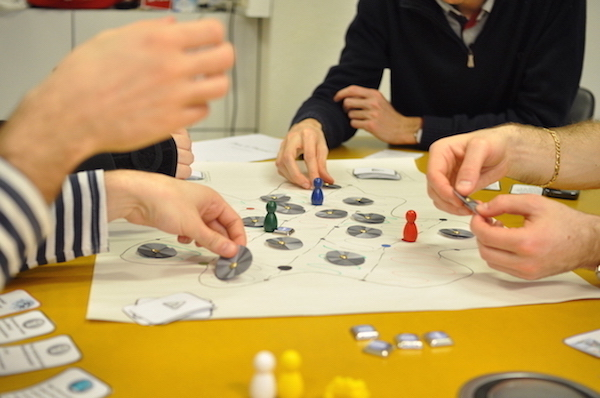
\includegraphics[width=1 
	\textwidth]{dp_mockup} \caption{Paper mockup of “Dont’ Panic!”} \label{fig:dp-mockup} 
\end{figure}

This pilot study and the derived implication for design have driven the design of an technology-enhanced version of the game presented in P5.

\emph{Relation to the research questions: } The paper contributes to the investigation of RQ2, ``\RQii''

\section[The interactive-token approach to board games]{Paper 5}\label{paper-5}

\emph{Title:} The interactive-token approach to board games

\emph{Authors:} Simone Mora, Ines Di Loreto and Monica Divitini

\emph{Authors' contributions:} Mora led the design and implementation work. He was also the~main~contributor of the paper. Di Loreto designed the board game that is used as example in the paper. Di Loreto and Mora jointly designed and attended evaluation studies.~Divitini provided~general~supervision for the research and the paper writing.

\emph{Published in:} Ready for submission 
\begin{quote}
	\emph{Abstract:} Recent advances in interactive surfaces and Tangible User Interfaces have created a new interest in digital board games, aiming at mixing the benefits of traditional board games with the interactivity of video games. Within this strand of research we propose a new approach centred on the concepts of tokens, constraints, spatial expressions and interaction events. While mainstream solutions implement game interaction using interactive surfaces, our approach relies on physical manipulation of interactive objects on conventional surfaces. We illustrate the proposed approach by describing the design and development of a game for training of emergency workers. Building on feedbacks from user evaluation and our experience with the development, we outline design opportunities and challenges of the approach. 
\end{quote}

\emph{Description:} The paper presents a novel approach to the digitalisation of board games. The approach aims at adding computer games interactivity preserving board games's traditional social and physical affordances. Rather than implementing games for interactive surfaces (e.g.~touch-screens) the approach relies on the physical manipulation of interactive objects on conventional surfaces. After reviewing state of the art technology for digital board games, the approach is presented and grounded in existing frameworks of tangible user interfaces. To facilitate implementation of the approach into the design practice of digital board games a three-steps process is presented. The process provides guidelines for designing computer-augmented game pieces and for mapping sensing-based interactions with pieces to game dynamics.

P4 introduced \emph{Don't Panic}, a serious game for enhancing soft skills for crisis workers, pointing out the role of technology as facilitator for generating engaging game experiences and for supporting post-game reflection and mapping with the real work. The approach and process presented in this paper have been used to drive a new design iteration for the game. 

In the new, technology-augmented prototype (Figure \ref{fig:dp-token}), social affordances of traditional board games, in terms of prompts for cooperation and discussion, are preserved. This is functional to the serious role of \emph{Don't Panic} as facilitator for storytelling and team building. At the same time the added computer interactivity provides a game experience which is more immersive and less disrupting compared to the paper mockup presented in P4. This allows for generating, by means of the game, a simulated work experience (management of panicking crowds) that re-create as much as possible conditions of emotional stress and decision making under time constraints, typical of real work. The prototype has been evaluated against usability with 16 players who played the game in groups of four. Results from the experiment contribute in shedding the light on opportunities and challenges offered by the presented approach.

The paper also describes the technical challenges faced by the authors during the prototyping process. A mix of software, hardware, laser-cut and 3D printing techniques have been orchestrated in order to fully implement game dynamics and produce a prototype of a game that can be played for an entire session without major disruptions. Beside allowing to implement a new version of \emph{Don't Panic} the approach proposed in the paper is a contribution in the field of TUIs which can inspire the design of new digital board games.

\begin{figure}
	[tbh] \centering 
	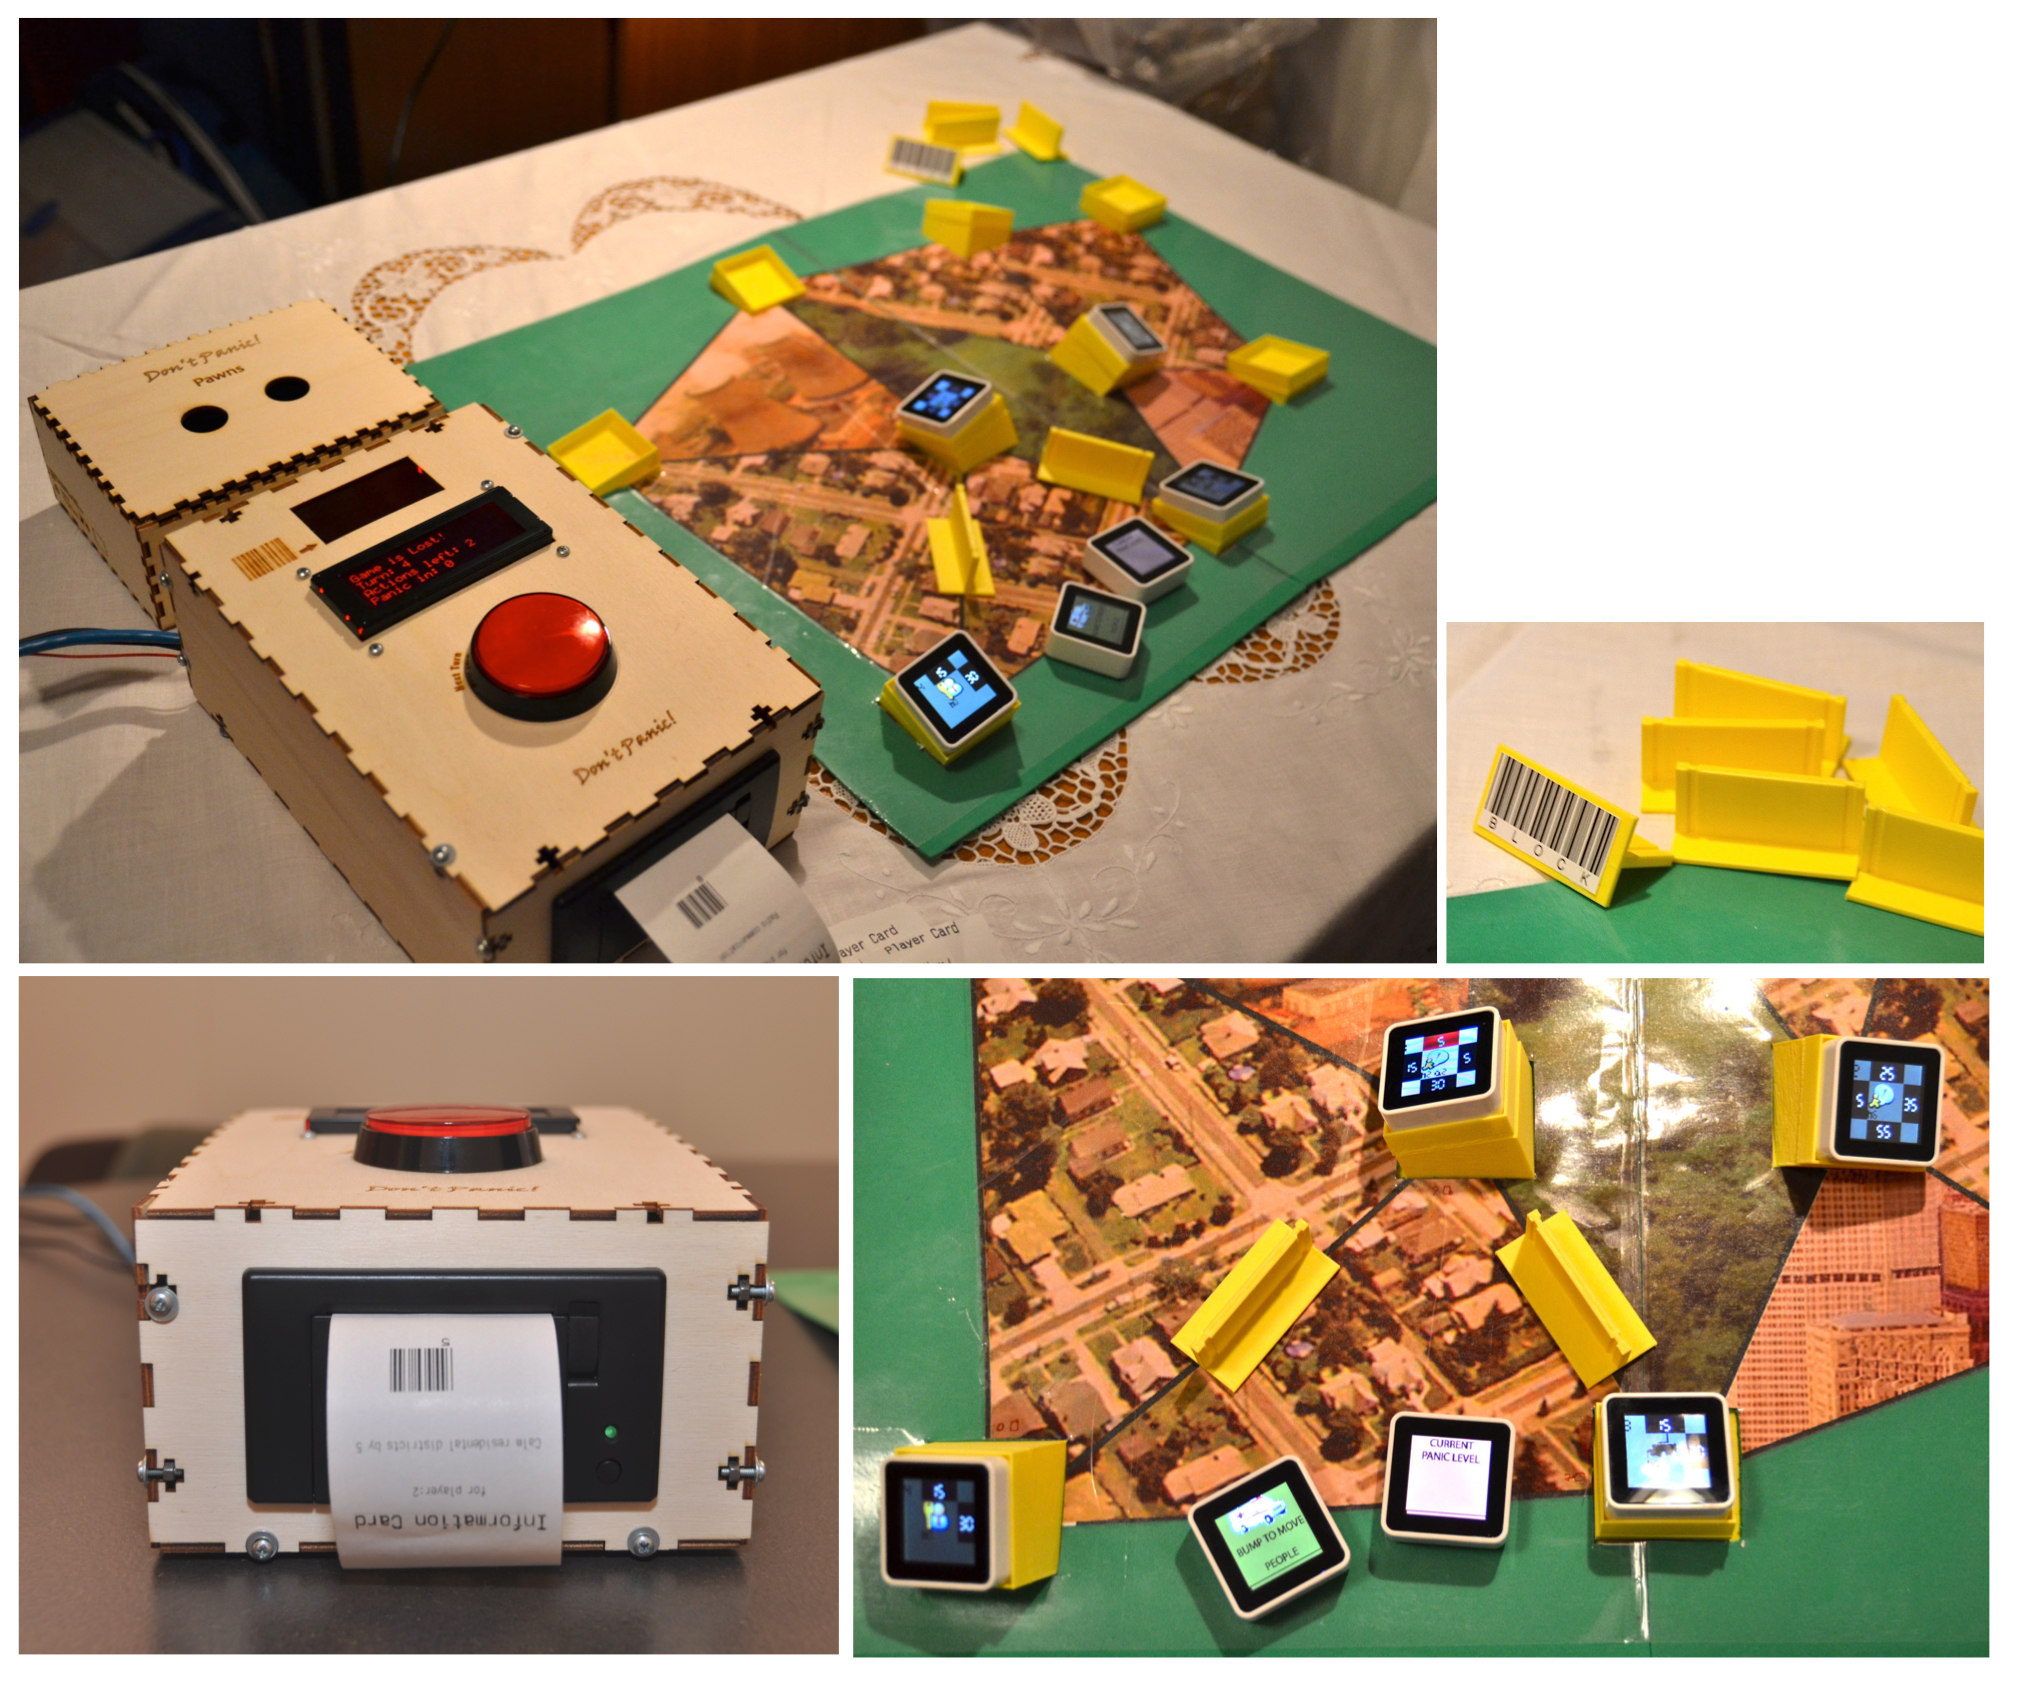
\includegraphics[width=1 
	\textwidth]{dp-multi} \caption{Technology-augmented “Don't Panic!” working prototype} \label{fig:dp-token} 
\end{figure}

\emph{Relation to the research questions: } The paper contributes to the investigation of RQ2, ``\RQii'' and RQ3, ``\RQiii''

\section[Context Becomes Content: Sensor Data for Computer-Supported Reflective Learning]{Paper 6}\label{paper-6}

\emph{Title:} Context Becomes Content: Sensor Data for Computer-Supported Reflective Learning

\emph{Authors:} Lars Müller, Monica Divitini, Simone Mora, Verónica Rivera-Pelayo and Wilhelm Stork

\emph{Authors' contributions:} Müller led the writing of the paper and contributed with one of the case studies. Mora designed the systems presented in the second case study. Mora also designed and conducted the evaluation of the system. Rivera-Pelayo contributed with state of the art about~the quantified self and to the methodological part. All the authors contributed to draw lessons learned and theoretical implications~from~the two~studies. Divitini and Stork contributed with supervision during the writing process.

\emph{Published in:} IEEE Transactions on Learning Technologies 
\begin{quote}
	\emph{Abstract:} Wearable devices and ambient sensors can monitor a growing number of aspects of daily life and work. We propose to use this context data as content for learning applications in workplace settings to enable employees to reflect on experiences from their work. Learning by reflection is essential for today's dynamic work environments, as employees have to adapt their behaviour according to their experiences. Building on research on computer-supported reflective learning as well as persuasive technology, and inspired by the Quantified Self community, we present an approach to the design of tools supporting reflective learning at work by turning context information collected through sensors into learning content. The proposed approach has been implemented and evaluated with care staff in a care home and voluntary crisis workers. In both domains, tailored wearable sensors were designed and evaluated. The evaluations show that participants learned by reflecting on their work experiences based on their recorded context. The results highlight the potential of sensors to support learning from context data itself and outline lessons learned for the design of sensor-based capturing methods for reflective learning. 
\end{quote}

\emph{Description:} This paper proposes the use of context data as content to support reflective learning in workplace settings. The approach uses technology to turn unstructured context data into learning contents. Two case studies presented in the paper demonstrate how the approach facilitates designers in mapping requirements from reflective learning theory with opportunities provided by technology, within the constraints of the specific workplace environment.

Three design decisions have to be made to turn context into content: \emph{what context} is relevant to be captured, \emph{how to capture} it and \emph{how to visualise} it to support reflection. The first two decisions were already explored drafting design challenges for data capturing tools (P3). In this paper they are further elaborated.

The paper reveals that the decision of \emph{what context} to be captured is highly situated with the work experience to be acquired. The decision is made harder by the unpredictability of outcomes typical of the reflective practice and by the need for interpretation required by the unstructured nature of context data. Yet the paper identifies three types of context that may include relevant data for reflection: \emph{task}, \emph{affective} and \emph{social}. \emph{Task context} relates directly to the work process and is therefore easy to understand. \emph{Affective context} might work as a marker to recognise relevant episodes for reflection; because if something happens during the day, it will trigger an emotional reaction that can be captured with sensors. Finally \emph{social context} is important for many collaborative work practices since the interactions with other people (colleague, customers, patients) constitute an important aspect of many experiences to reflect upon.

\emph{How to capture context} is also further elaborated in this paper. Three methods are proposed. Data can be \emph{self-reported} by the users, thus providing a subjective impression on an experience (e.g. by means of digital diaries). Data can be \emph{self-reported from third parties} in this way an external perspective is made available to the reflecting person. Finally data can be captured \emph{automatically} by sensors and applications; for example by means of stress or activity-tracking sensors.

Compared to P3 the paper adds a third design challenge connected to \emph{visualisation of context}. In order to be effective in triggering and sustaining a reflection sessions, data should be visualised from multiple perspective. Discrepancies among different view of the same experience should be outlined as reflection triggers. The social (comparing data over multiple users), spatial (the location data were captured) and historical perspectives (evolution of data samples over time) are considered as effective for reflection. The CroMAR app (P1) and Trainer app (P2) were designed to visualise data according with one or more of those perspectives.

The three design dimensions are functional to build technology tools that implement the stages of the CSRL cycle (Chapter \ref{csrl}). While what context and how to capture it pertains designing of technology to support the \emph{plan and do work} stage of the model, \emph{how to visualise data} provides support for the subsequent stages of \emph{initiate reflection} and \emph{conduct reflection session}. To motivate the user in the data collection process methods borrowed from persuasive technology and quantified self are presented.

The paper further presents two case studies and their evaluation. One of the cases show the use of WATCHiT (P3) and Trainer (P2) to support reflection on the implementation of protocols (e.g.~medical procedures) by workers in the field, immediately after the procedure is performed. The system promotes a quick reflection session with easy triggers that can be done by the worker herself or collaboratively by a team. The second case study is an application designed to support carers in dementia care homes by reflecting on their daily interaction with residents and colleagues. Both case studies have target users -carers and crisis workers-, that work in highly dynamic environments and therefore benefit the most from on-the-job, reflective training.

Field evaluations for two case studies show that participants were able to learn from the visualised context. Yet, it is confirmed that learning goals and expected outcomes are difficult to be defined a priori. It is also considered important to provide an option to record reflection outcomes, so that the gained insight can be user later (and might trigger new reflection cycles). Capturing tools should be easy to adapt, in order to allow the users to deal with the unpredictability of relevance of the captured context. This choice has been implemented in WATCHiT (P3) by means of physical sensor modules.

\emph{Relation to the research questions: } The paper dresses RQ1 ``\RQi'' and RQ2, ``\RQii''

\section[A Unified Architecture for Supporting Direct Tag-Based and Indirect Network-Based Resource Discovery]{Paper 7}\label{paper-7}

\emph{Title:} A Unified Architecture for Supporting Direct Tag-Based and Indirect Network-Based Resource Discovery

\emph{Authors:} Simone Mora and Babak Farshchian

\emph{Authors' contribution:} Mora conducted the design work and wrote the paper. Farshchian provided feedbacks throughout both the design and writing processes.

\emph{Published in:} Proceedings of the European Conference on Ambient Intelligence (AMI), 2010 
\begin{quote}
	\emph{Abstract:} Discovering and integrating ambient computational resources is a central topic in AmI. There are two major existing approaches: indirect network-based resource selection and direct tag-based resource identification. We motivate the need to integrate the two approaches through a scenario. We then present an architecture for a pluggable discovery system called UbiDisco. We demonstrate how UbiDisco implements a seamless integration of the two approaches at user interaction level through a framework for implementing discovery actions. 
\end{quote}

\emph{Description:} This paper presents a modular approach to software components for service discovery that blends the benefits of direct tag-based and indirect network-based discovery. The approach has been implemented in a middleware, called \emph{UbiDisco}, that allows for discovery and customisation of computational resources and support data exchange between heterogeneous systems. \emph{UbiDisco} is both a middleware and a collection of user interfaces for service discovery.

The work constitute a foundation of the rapid prototyping approach pursued in this PhD. As demonstrated in P2 and P6 the CSRL cycle is supported by a set of diverse technologies spanning from wearable and physical computers to apps for tablets and smartphones. Enable workers to easily link those tools in order to allow data exchange is critical to build custom, scenario-specific ecologies of tools to support the different stages of the reflection cycle. Integrating different apps is technically complex since it involves serialisation of data, configuration of wireless networks and interaction of back-end services such as databases. From the perspective of the user it involves filling in configuration details. This activity might be very complex on mobile and wearable tools.

UbiDisco hinders the user from the complexity of configuring technical details by means of \emph{discovery actions}. The user can link two systems by reading a barcode or RFID tag which identifies the device/service and provide technical details for the configuration of the link. For example CroMAR running on a iPad can be linked to WATCHiT, by reading a barcode printed on the device hardware. In this way WATCHiT and CroMAR network addresses and protocols in use are exchanged between the two systems. WATCHiT becomes a data provider for CroMAR until a new \emph{discovery action} links WATCHiT to a new system (e.g.~another instance of CroMAR or Trainer).

\emph{Relation to the research questions: } The paper contributes to RQ3, ``\RQiii'' 

\chapter{Contributions}\label{contributions}

\todo[inline]{Revision 3:\\-updated description of contributions \\ -added tables}

The contributions of this PhD work are presented according to four areas:

\begin{enumerate}
	\def\labelenumi{\arabic{enumi}.} 
	\itemsep1pt\parskip0pt\parsep0pt 
	\item \Ci 
	\item \Cii 
	\item \Ciii 
	\item \Civ
\end{enumerate}

Contribution 1 maps CSRL theory with applications of technology, contribution 2 provides design challenges for experience-capturing tools, contribution 3 relates to the design of novel interaction techniques to fit systems' requirements emerged during field studies. Finally contribution 4 sheds the light on challenges for rapidly implement design ideas in working prototypes.

Table \ref{tab:papers-and-contributions} summarises the contributions provided by the papers.

\begin{table}[tbh] 
	\centering 
	\caption{Papers' additions to the contributions} 
	\label{tab:papers-and-contributions} 
	\smallskip
	\begin{tabular}{@{}lcccc@{}}
	\toprule
	  & \begin{turn}{90}Contribution 1\end{turn} & \begin{turn}{90}Contribution 2\end{turn} & \begin{turn}{90}Contribution 3\end{turn} & \begin{turn}{90}Contribution 4\end{turn} \\
	\midrule
	Paper 1 & & & \textbullet & \\
	Paper 2 & \textbullet & \textbullet & & \\
	Paper 3 & & \textbullet & \textbullet & \textbullet \\
	Paper 4 & \textbullet & & & \\
	Paper 5 & & & \textbullet & \textbullet \\
	Paper 6 & \textbullet & & & \\
	Paper 7 & & & & \textbullet \\
	\bottomrule 
	\end{tabular}
\end{table}

\section{C1: Implementation and evaluation of MIRROR Computer Supported Reflective Learning (CSRL) theory}\label{c1}

Contribution 1 of the thesis comprises new knowledge about how theoretical concepts in the CSRL model (Chapter \ref{csrl}) can be mapped to technologies and implemented in artefacts. The work provided successful applications of technologies, in crisis training, that constitute an empirical evaluation of the model itself.

The CSRL model developed by Krogstie et al. \autocite*{Krogstie:2013kf} (Figure \ref{fig:csrl-model-contrib}), presents a cycle of four stages to conceptualise reflection at work. For each stage a set of reflection-useful activities that can be enhanced by technology are presented. 

\begin{figure}
	[tbh] \centering 
	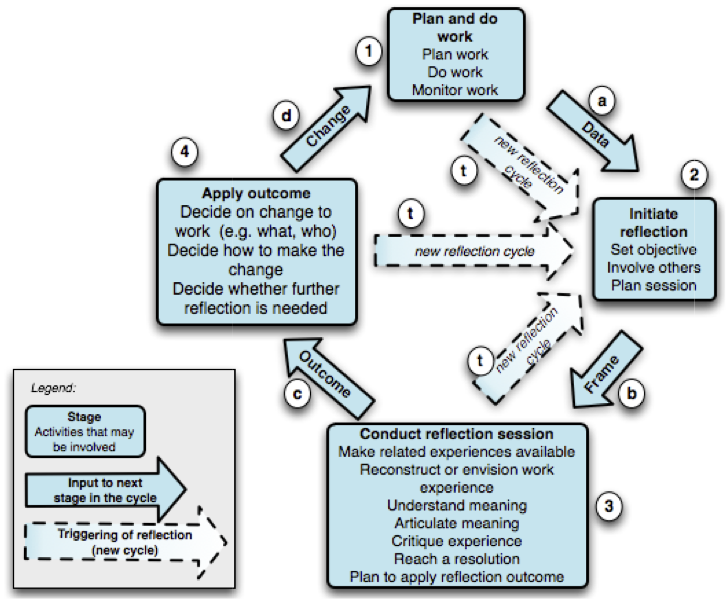
\includegraphics[width=1
	\textwidth]{CSRL} \caption{CSRL reflection cycle. Figure adapted from \protect\autocite{Krogstie:2013kf}} \label{fig:csrl-model-contrib} 
\end{figure}

During this PhD specific activities from the four stages of the model have been supported with technology tools (Table \ref{tab:model-instantiation}). 

\begin{table}[tbh] 
	\centering 
	\caption{Instantiation of the CSRL model} 
	\label{tab:model-instantiation} 
	\smallskip
	\begin{tabular}{@{}P{0.15\linewidth}P{0.35\linewidth}P{0.20\linewidth}P{0.20\linewidth}@{}}
	\toprule
	Stage & Activity & Technology & Prototype \\
	\midrule
	Plan and do work & Do work & Digital board game & \emph{Don't Panic} \\
	                 & Monitor work & Wearable computers & \emph{WATCHiT}  \\
	\hline
	Initiate reflection & Involve others & Mobile augmented & \emph{CroMAR} \\
	Conduct reflection  & Make related experiences available & reality  &  \\
	session & Reconstruct or envision work experience &  & \\
	& Understand meaning &  \\
	& Articulate meaning &  \\
	& Critique experience &  \\
	Apply  & Decide on change to work & \\
	outcome & Decide how to make the change & \\
	\bottomrule 
	\end{tabular}
\end{table}

Although different prototypes focus on supporting different activities, they can be combined (as described in P2) in order to provide full support to the CSRL cycle. 

During the \emph{plan and do work} the \emph{monitor work} and \emph{do work} activities have been supported. The \emph{monitor work} activity has been implemented by \emph{WATCHiT} (P3) which empowers workers for capturing a wide spectrum of qualitative and quantitative data. I found out that \textbf{wearable sensor technology and embodied user interfaces} provide the best design choice for data collection. The \emph{do work} activity has been supported by \emph{Don't Panic} (P4, P5), by generating realistic work experience that push workers towards taking actions common of real work and under stress conditions in a game environment. Although the \emph{do work} phase in the model describes real work activities, for the specific case of crisis management we claim it can also be applied to simulated work. Indeed, the innovative \textbf{digital board game technology} presented in P5 was effective in recreating stress conditions similar to real work and collaboration affordances typical tho the ones observed during field studies.

The \emph{Conduct reflection session} \emph{CroMAR} (P1) supports a wide range of activities. First it makes \emph{related experiences available} by aggregating data from multiple sources, including work experience of colleagues (captured by \emph{WATCHiT}), social networks and open data. Then \emph{CroMAR} allows for visualising data while being situated in a physical context that helps to \emph{reconstruct or envision work experience}. By allowing layering and filtering of data according to source, time and space it facilitates to \emph{understand and articulate meanings}. Finally an embedded text editor allows for the collection and sharing of lesson learnt and to elaborate a plan to apply reflection outcomes. Thanks to the experience with \emph{CroMAR} we also found out that \textbf{mobile augmented reality technology} is efficient in supporting debriefing and reflection after crisis work.

Contribution 1 can be a resource for researchers in the field of computer supported reflective learning that strive in finding solutions to map theory tools to technologies that people can use at work. Although the applications developed are tailored to the crisis training domain, they could be redesigned for other domains. The need for pervasive data collection and disruption-free interfaces is shared by many work practices; the digital board game approach developed in P5 has been proven to be a useful tool also in generating realistic work experience for the dementia care domain, as investigated during research work abroad (see Appendix \ref{abroad}). Finally a new application domain for mobile augmented reality technology: to support debriefing. \emph{CroMAR}, the tool developed in P1, could be adapted to support debriefing of work practices that share similarities with the crisis domain. The presented technology tools constitute an empirical evaluation of theory which outcomes (P2,P6) can inform future development of the CSRL model. Finally a new approach to the design of technology to turn unstructured context data into learning contents was presented in P6 and evaluated across two cases studies. The approach aims at extending the body of knowledge in computer-supported reflective learning.

\section{C2: Knowledge about designing experience-capturing tools for crisis workers}\label{c2-knowledge-about-designing-experience-capturing-tools-for-crisis-workers}

Contribution 2 of this thesis is a set of challenges for the design of experience-capturing tools during real or simulated crises.

Seven design challenges derived from multiple user studies with crisis workers, have been reported in P3. The challenges are summarised in Table \ref{tab:design-challenges}. Despite there are guidelines for designing sensor and capturing tools for a variety of domains; in this work I focused on capturing information that is is relevant for reflective learning in crisis training. The challenges shed light on \emph{what} information is relevant and \emph{how} to capture relevant information. This contribution also highlights a design trade-off common for many sensing-based applications: the degree of data that can be captured with sensors, automatically and without user intervention, versus information that can be submitted in-action by workers themselves; which, in the case of crisis training, requires novel interaction approaches (Contribution 3). 

The challenges have informed the design of \emph{WATCHiT}, a modular data capturing tool (P3) that has been successfully evaluated in a scenario to support debriefing after procedural training (P2). \emph{WATCHiT} can be configured to address new scenarios, data captured can be also used to support coordination of work or monitoring activities in real time.

Contribution 2 can be a resource for computer scientists aiming at designing technologies for pervasive quantitative and qualitative data collection. The presented challenges constitute a foundation for a design space for data capturing tools. They are an expression of the trade-off between technology-centred quantitative data acquisition and user-centred qualitative information collection.

\begin{table}
	[p] \centering \caption{Design challenges for data collection tools in crisis work} \label{tab:design-challenges} 
	\begin{tabular}
		{@{}p{0.05\linewidth}p{0.25\linewidth}p{0.60\linewidth}@{}} \toprule & Challenge & Description \\
		\midrule DC1 & Mobility of work and sensing & It is important to complement data from sensors embedded in the environment with mobile ones. The degree of mobility and thus granularity of data is important. Fine granular data is achieved with sensors worn by first responders. \\
		DC2 & Different crises, different relevant data & Being each crisis almost unique, it is difficult to define which data might be relevant to capture based on generic typologies of crises. \\
		DC3 & Different types of data & Different types of information are relevant to be captured. Including information for assessment of the worker’s safety, for mapping the territory and the work and Information related to the rescued people (e.g. type of injures). \\
		DC4 & Sensor data and user-submitted data & Workers might however provide critical qualitative data that cannot be measured with sensors to complement quantitative ones. \\
		DC5 & Different use, different sharing & While some types of data (e.g. location of agents) can be shared with colleagues to support real-time real time coordination, it's up each agent whether to share or not sensitive data (e.g. stress levels) with peers. \\
		DC6 & Intuitive, hands-free interaction & Workers must focus on the rescue operation and not on data capturing and logging tasks. User interfaces must be very intuitive and distraction-free. \\
		DC7 & Automate and discrete capturing & Capturing data with automatic means doesn't require user intervention but it produce datasets often affected by noise. Discrete capturing requires the user to activate sensors but produces more relevant and contextualised data. \\
		\bottomrule 
	\end{tabular}
\end{table}


\section{C3: Novel sensing-based interaction techniques to support recreation and generation of work experiences in crisis training}\label{c3-novel-sensing-based-interaction-techniques-to-support-recreation-and-generation-of-work-experiences-in-crisis-training}

Contribution 3 of the thesis brings novel interaction techniques to the field of sensing-based interfaces.

The interaction techniques developed assist different tasks.

During \emph{capturing work experience} the focus is on empowering users for collecting work experience without disrupting the work (due to interaction with the capturing tool). Building on prior works on mnemonic shortcuts \autocite{Guerreiro:2008wt} and body-centric interaction \autocite{Chen:2012wk} in P3 a novel disruption-free user interface is presented. It allows to use predefined body areas and objects as mnemonic shortcuts to activate sensors and to tag quantitative data with user-predefined information.

To enhance \emph{re-creating work experience} \emph{CroMAR}, the system presented P1, leverages mobile augmented reality (MAR) to enable visualisation and manipulation of reflection-useful information while being co-located in a physical context. In the implemented system the use of MAR technique has been proven successful in triggering reflection (P2). Moreover usability issues typical of MAR applications (e.g.~information overloading or occlusion visualising huge datasets) have been tackled by providing mechanism for filtering the information visualised according with time and source.

Finally during \emph{generating working experience}, tangible user interface frameworks have driven the design of the digital board game presented in P4 and P5. Board game mechanics have been functional to generate realistic work experience in terms of collaboration affordances and decision making. In this setting the use of tangible and sensing-based interaction added realism to the experience and increased players engagement and fun. The game design presented in P4 has been generalised in a approach and design process,presented in P5, that will drive the creation of future digital board games.

Contribution 3 can be a resource for interaction designers interested in creating interfaces for disruption-free data collection of experiences, situated data visualisation and simulated interactive experiences. The interaction techniques developed can be translated to new application domains.

\section{C4: Knowledge about implementing prototypes to be deployed into the wild}\label{c4-knowledge-about-implementing-prototypes-to-be-deployed-into-the-wild}

Contribution 4 brings new knowledge derived from the experience of the author in constructing prototypes of hardware and software systems. Prototypes were developed from the early phases of the research work to be used as demonstrator of tools for data collection (C2) and novel interaction techniques (C3). Also, ecologies of prototypes were functional for the evaluation of the CSRL model (C1), when more than one prototype was orchestrated in order to support part of the CSRL cycle.

Eight prototypes have been developed as part of this thesis. Each of them involved a mix of software, hardware and casing design. From a software point of view, the challenges consisted in making heterogeneous systems to discover each other and exchange data over a common protocol. This challenge has been addressed by the \emph{UbiDisco} middleware developed in P7. Most of the prototype featuring embedded hardware, I iteratively developed relatively complex electronics; for example to sense data from the environment or to provide haptic and visual feedbacks. I employed a wide range of technologies and toolkits which were not designed to be integrated, highlighting potentiality and limitations of state of the art technology for embedded systems. For example, the system of P5 involved the use of three different hardware toolkits and programming languages, and a bit of hacking. This attitude hacking and tinkering existing toolkits has been required because a product to fully fulfil the implementation of requirements of our system was not available on the market. Yet this is a resource for hardware engineers willing bring advances in the state of the art of toolkit for building electronics.

Prototypes used by crisis workers, in-action, have to be built for higher resilience compared to digital artefacts developed for lab testing. The simulated rescue work activities in which we staged our systems' evaluations are designed to recreate conditions as close as possible to real emergencies; including exposure to physical and thermal shocks. This setting has required the prototyping process to move one step closer to product engineering. The final stage of prototypes feature 3D-printed and laser-cut enclosures to shelter the electronics from the environment. Moreover for iteration after iteration the size of the prototypes has shrunk. For example the system in P3 have reached in four iterations a size compatible for being comfortably worn underneath work uniforms.

Contribution 4 is a resource for hardware and software engineers. Also it serves at case study for researcher to investigate the design of hardware and software toolkits to assist prototyping of electronic inventions. 

\chapter{Evaluation}\label{evaluation}

\todo[inline]{Revision 3}

This chapter provides an evaluation of the contributions of the thesis with respect to research questions. In addition, validity threats are discussed in the chapter.

\section{Evaluation of Research questions}\label{evaluation-of-research-questions}

\subsection{MRQ: \MRQ}\label{mrq-what-are-the-opportunities-introduced-by-combining-reflective-learning-theories-with-sensing-based-interfaces-for-supporting-crisis-training}

The main research question is answered by Contribution 1. Using crisis training as case study for design research, it is demonstrated how conceptual tools from theory in CSRL can be implemented in a suite of applications of sensing-based technology: \emph{WATCHiT}, \emph{CroMAR}, and \emph{Don't Panic}. Each application assists specific activities which the CSRL model has identified to be relevant for reflection. Two or more applications can be configured to work together in an ecology, in order to address the interrelated nature of CSRL activities in terms of sharing of data and reflection outcomes. In this way it is also addressed the need for supporting the extremely vast range of scenarios workers train for by means of loosely coupled, modular applications.

\subsection{RQ1: \RQi}\label{rq1-how-sensing-based-interfaces-can-be-designed-to-enable-unobtrusive-experience-collection-during-crisis-work}

This question is answered by Contribution 2 and Contribution 3. C2 has identified a set of challenges for the design of experience-capturing tools, focusing on \emph{what} data to collect and \emph{how} to collect it. One of the identified challenges, the need of intuitive and hands-free user interfaces for capturing user-submitted qualitative information, has been further addressed by C3 with the design of a novel user interface for controlling the data capture process.

\subsection{RQ2: \RQii}\label{rq2-how-sensing-based-interfaces-can-be-designed-to-trigger-reflection-via-re-creation-or-generation-of-work-experiences}

This question is answered by Contribution 3. It is found out that theories in the field of tangible, embodied and embedded computing can drive the design of sensing-based interfaces either to \emph{capture work experiences} and to \emph{generate work experiences}. The specific paradigms adopted are mobile augmented reality, body-centric interaction and token+constraint interaction. Once more it is not a single interaction modality that has been proven to engage reflection but rather a mix of different technology-assisted experiences.

\subsection{RQ3: \RQiii}\label{rq3-how-sensing-based-interfaces-for-supporting-reflection-can-be-rapidly-prototyped}

This question is answered by Contribution 4. It is found out that prototyping sensing-based interfaces for supporting reflection require a wide range of skills ranging from software and electronic engineering. Yet a toolbox for assisting in full the work of designers and engineers in implementing functional requirements in prototypes couldn't be found. Despite so recent advances in open source hardware and software, digital manufacturing and technology developed by the author (P7) allowed the author to build working prototypes robust enough to undergo evaluations during simulated crisis work. Still the production of prototypes requires resources and skills not usually required for prototyping ``traditional'' ICT systems.

\section{Evaluation of research approach}\label{evaluation-of-research-approach}

The research approach taken in this thesis has a number of limitations. In this section validity issues are discussed.

\subsection{Conclusion validity}\label{conclusion-validity}

Conclusion validity questions whether the method used shows a relationship between the variables that are studied.

In this work the impact on reflective learning for the technology tools developed was evaluated (as proof of validity for C1). Also due to the novel nature of the user interfaces developed, technology acceptance tests and usability evaluations have been performed.

Considering the design research approach taken and the the number of human factors involved, methods from qualitative research were used in the evaluations. The methods used included observations, semi-structured interviews, surveys and questionnaires. The adoption of the MIRROR Evaluation Toolbox \autocite{Renner:v4nLmwOk}, which provided questionnaires to measure reflective learning at work, straighten the conclusion validity of the research. These questionaries are built on the Kirkpatrick framework \autocite{kirkpatrick2009evaluating} and have been developed through an extensive survey of literature on reflective learning and in cooperation with participants from different workplace settings.

The number of participants in the studies added up to 56 crisis field workers (e.g.~firefighters, paramedics), 1 disaster manager, 8 IT students and 4 HCI experts. Among the field workers 5 participants attended more than one study. The size of data samples used for statistical analysis is therefore limited and it weakens the conclusion validity, especially for the evaluation studies for the applications targeting disaster managers (CroMAR). Furthermore most of evaluation studies lasted only for a few hours. It is therefore not possible to asses long-term learning effects for the solutions developed.

\subsection{Internal validity}\label{internal-validity}

Internal validity questions whether the method used demonstrates a casual relationship between two variables or not.

By running field studies during physical simulations arranged by external organisations, most variables couldn't be controlled. Access to workers and locations where the work is performed was restricted to avoid obstructing activities, explosing training objectives of the events and attendees' safety at risk. Despite the good will of simulations' attendees and organisers, it wasn't always possible to fully attend to the evaluation protocol agreed due to both planned and unplanned unpredictability of such events.

Yet the lack of control was traded for realism. Events attended recreated working conditions as close as possible to real emergencies. Participants were unaware of the type of emergency to face until the very last, human mistakes and failure of technical systems were re-created on purpose by the event manager. Finally, during the observed events, volunteers acting as injured were made-up with fake wounds and instructed to behave accordingly (e.g.~panicking). Considering the very situated nature of crisis work, the widespread layout of activities in space, the coexistence of multiple roles and organisations, choosing field studies over an experimental strategy has strengthen the internal validity of the work. Giving for granted that running field studies during real crisis work is not feasible due to safety reasons.

\subsection{External validity}\label{external-validity}

External validity questions whether the relationship found can be generalised to other settings.

Given the characteristics of the sample of population the research has been evaluated with, it is not possible to draw conclusions about generalisations of results, both within the crisis domain and to other settings.

First, participants of field studies performed are all affiliated to a small set of crisis response organisations; the design research has been case studied on the specific needs of those organisations. Although a review of literature have shown that technology requirements found in our user studies are common to other organisations in different countries, it is not given to know how the results from this work could be accepted by other organisations. This weakens the results of research. Contacts with external organisations have been established in order to evaluate generalisation of results as part of future works.

Second, it hasn't been thoroughly investigated how results from this PhD could be translated to work practices different than the crisis domain. The novel interaction techniques and the rapid prototyping approach developed have been employed to create games for training workers in dementia care homes for better care, during a research visit abroad. The same approach drove the design and implementation of tangible interface to promote user engagement and reflection about urban-mobility data, as part of a second research visit abroad (Appendix \ref{abroad})

\subsection{Reliability}\label{reliability}

Reliability is the extend to which another researcher would find the same answers.

Most of the data were only observed, recorded and analysed by one person, which is subject to interpretation bias. However some of the data were analysed by two or more people. Further, different researchers have been responsible for different studies. 

\chapter{Conclusions and future works}\label{conclusions}

\todo[inline]{Revision 3}

This thesis has focused on enhancing crisis training practices with novel sensing-based technologies to capture, re-create and generate crisis work experiences.

The main research method adopted was design science. To this respect six field studies during physical simulations of crisis work were performed. Field work and literature in computer-supported reflective learning has driven eight prototyping iterations during which fairly complex hardware/software sensing-based devices were built and evaluated both in focus groups and on the field. The work has resulted in seven paper published and five declaration of inventions filed for technology transfer.

The research questions were answered by four contributions, hereafter summarised in a set of conclusions which delineate future works. \bigskip

\emph{Contribution 1} 
\newline \rule{
\textwidth}{.1pt} \emph{The MIRROR CSRL model (Chapter \ref{csrl}) can be used to technology-enhance reflective learning practices in crisis training. Activities described in the model together with requirements derived from field studies drove the design of sensing-based interfaces to support the capture, re-creation and generation of work experiences. Eight prototypes were built, including wearable data-collection tools (P3), mobile augmented reality browsers (P1) and serious games (P4,P5). Ecologies of prototypes were successfully evaluated for their impact in supporting debriefing after physical simulations of crisis work (P2). New theories about the use of sensor data as learning content emerged (P6).}

Further work is required to map with technology the two stages in the model not addressed in this research work. As evaluated in Chapter \ref{evaluation}, the investigation in this thesis is deeply connected with the specific case of crisis work. Future works will generalise the theoretical findings and the technologies produced to other domains. \rule{
\textwidth}{.1pt} \medskip

\emph{Contribution 2} 
\newline \rule{
\textwidth}{.1pt} \emph{Capturing relevant data to feed reflection processes is challenging due to the unpredictability of relevance typical of reflection (P6). In addition, the highly dynamic nature of crisis work requires to design tools that need to be adapted to the  needs of always varying scenarios. This space of opportunities is provided to researchers as a set of challenges to the design of experience-capturing tools (P3). The challenges were explored with the development of data collection tools that can be used to support debriefing (P2). Prototypes developed feature wearable sensors and an embodied user interfaces based on mnemonic body shortcuts.}

Further work is required to validate the identified challenges with more field work and to investigate challenges not addressed in this work production of prototypes. Furthermore the relevance of the challenges to other application domain has to be investigated. \rule{
\textwidth}{.1pt} \medskip

\emph{Contribution 3} 
\newline \rule{
\textwidth}{.1pt} \emph{Novel approaches inspired by the field of tangible, embodied and embedded computing can facilitate interaction with technology to support reflection. The approaches have driven the design of interfaces to reduce distraction while interacting with capturing tools during work, to allow for browsing information in physical environments that contextualise reflection; and to provide social and engaging serious gaming experiences.}

Further work points at validating the developed approaches with the production and evaluation of new prototypes; and to further formalise interaction models and design processes.

\rule{
\textwidth}{.1pt}

\medskip

\emph{Contribution 4} 
\newline \rule{
\textwidth}{.1pt} \emph{Prototypes have a central role in design science research for the validation of theories and in the development of new methods. Yet, prototyping sensing-based interfaces require large efforts due to the wide range of skills required, including hardware and software engineering, product design and assembly. Further, technology artefacts to be tested during crisis work are to be built for higher resilience compared to the ones deployed for lab testing. Despite prototyping toolkits are available, to date an holistic tool to support the development of both software and hardware complex features couldn't be found. This has resulted in large efforts required for building prototypes and in the development of a understanding of the challenges and tools currently available.}

Future work builds on the challenges experienced with the production of prototypes for this PhD work for the conceptualisation and production of a toolkit to ease the production of complex sensing-based systems. 
\rule{
\textwidth}{.1pt}
\bigskip

In conclusion, this thesis has developed knowledge about the implementation of computer supported reflection theories into novel ICT systems and sensing-based interfaces that can produce learning outcomes. Although the investigation is limited to the characteristic case of crisis training, basis for the generalisation of theories and technologies developed have been settled. Commercial exploitation of research outcomes is being explored, research funds have been granted to this purpose (see Section \ref{exploitation-of-research-contributions}). Future works aim at generalising research findings to new domains and to commercially exploit research results. 


\appendix
\chapter{Research Papers}\label{papers}

\textbf{Paper 1} Mora, S., Boron, A., \& Divitini, M. (2012). CroMAR:
Mobile Augmented Reality for Supporting Reflection on Crowd Management.
\emph{International Journal of Mobile Human Computer Interaction}, 4(2),
88--101. Available at: http://simonemora.me/papers/P1.pdf

\textbf{Paper 2} Mora, S., \& Divitini, M. (2014). Supporting Debriefing
with Sensor Data: A Reflective Approach to Crisis Training. \emph{In
Proceeding of Information Systems for Crisis Response and Management in
Mediterranean Countries, ISCRAM-MED}, 196(7), 71--84. Available at:
http://simonemora.me/papers/P2.pdf

\textbf{Paper 3} Mora, S., \& Divitini, M. (2014). WATCHiT: a modular
and wearable tool for data collection in crisis management and training.
\emph{In Proceeding of the European Conference in Ambient Intelligence,
AMI}, 8850(22), 274-289. Available at:
http://simonemora.me/papers/P3.pdf

\textbf{Paper 4} Di Loreto, I., Mora, S., \& Divitini, M. (2012). Don't
Panic: Enhancing Soft Skills for Civil Protection Workers. \emph{In
Proceeding of International Conference on Serious Games Development
Applications, SGDA}, 7528(1), 1--12. Available at:
http://simonemora.me/papers/P4.pdf

\textbf{Paper 5} Mora, S., Di Loreto, I., \& Divitini, M. The
interactive-token approach to board games. \emph{Ready for submission}.
Available at: http://simonemora.me/papers/P5.pdf

\textbf{Paper 6} Müller, L., Divitini, M., Mora, S., Rivera-Pelayo, V.,
\& Stork, W. (2014). Context Becomes Content: Sensor Data for Computer
Supported Reflective Learning. \emph{IEEE Transactions on Learning
Technologies}, PP(99). Available at: http://simonemora.me/papers/P6.pdf

\textbf{Paper 7} Mora, S., \& Farshchian, B. A. (2010). A Unified
Architecture for Supporting Direct Tag-Based and Indirect Network-Based
Resource Discovery. \emph{In Proceeding of the International Conference
on Ambient Intelligence, AMI}, 6439(20), 197--206. Available at:
http://simonemora.me/papers/P7.pdf

\chapter{Secondary papers}
\label{secondary-papers}

In this appendix papers which are not included in the PhD thesis are briefly summarised. The papers present work-in-progress or incremental achievements that have led to the research results reported in the thesis.

Each summary includes:

\begin{itemize}
	\item Title
	\item Authors
	\item Where the paper was published
	\item Brief description of the paper's contribution
\end{itemize}

\Section{Paper 1}

\emph{Title: }WATCHiT: Towards wearable data collection in crisis management

\emph{Authors: }Simone Mora and Monica Divitini

\begin{quote}
	\emph{Abstract: }In this paper we present the work-in-progress on WATCHiT, a wristband computer for data collection during crisis response work. We outline the user-centered research methodology we adopt and we identify four design challenges to be tackled. We report the design of a working prototype that relies on wearable sensors to capture quantitative data and on an eyes-free, token-based interface for tagging sensor data with user-defined text messages. The prototype has been evaluated with emergency workers during a simulated rescue operation.
\end{quote}

\emph{Published in: }Work-in-progress at the Eight International Conference on Tangible, Embedded and Embodied Interaction (TEI), 2014.

\emph{Description: }The papers present a first draft of the design challenges for experience-capturing tools and a description of a early prototype of \emph{WATCHiT}. 

\Section{Paper 2}

\emph{Title: }Supporting Crisis Training with a Mobile Game System

\emph{Authors: }Ines Di Loreto, Emil Mork, Simone Mora and Monica Divitini

\begin{quote}
	\emph{Abstract: } Crisis training is highly complex and it requires multiple approaches. Games have a high potential in this context because they might support players in exploring different situations and experience different crisis scenarios. This paper proposes a mobile game system for crisis training. The system aims to promote soft skills and basic procedures learning. The system is composed by (i) a website that allows to set up the game and review game results and (ii) a mobile game. The set up supports the tailoring of games that better fit the specific learning needs of the players. The actual play promotes gaining of experience. The final review is intended to promote reflection on the gained experience, mirroring debriefing sessions that are common in crisis situations. Results from the initial evaluation show that the game and the post-game reflection are useful to train soft skills and to improve behavior.	
\end{quote}

\emph{Published in: }Proceedings of the International Conference on Serious Games Development Applications (SGDA), 2013.

\emph{Description: }The game presented in the paper is a mobile version of the \emph{Don't Panic} board game, aiming at providing alike learning objectives, yet via a collaborative pervasive gaming experience.

\Section{Paper 3}

\emph{Title: }Token-based Interaction with embedded digital information

\emph{Authors: }Simone Mora

\begin{quote}
	\emph{Abstract: }Embedding digital information into places and objects can improve collaborative processes by allowing a piece of information to travel across different contexts of use. Yet tools for supporting the processes of information embedding, discovery and visualization are needed. This PhD-work aims at providing a conceptual framework that promote the use of (in)tangible tokens to enable information embeddedness. The framework is used to drive the design of pervasive applications to support collaboration and reflection in crisis management.
\end{quote}

\emph{Published in: }Doctoral consortium of the International Conference on Tangible, Embedded and Embodied Interaction (TEI), 2013.

\emph{Description: }This paper details a work-in-progress on the research questions and methodology adopted throughout the PhD work. It also describes early contributions.

\Section{Paper 4}

\emph{Title: }Tangible and Wearable User Interfaces for Supporting Collaboration among Emergency Workers

\emph{Authors: }Daniel Cernea, Simone Mora, Alfredo Perez, Achim Ebert, Andreas Kerren, Monica Divitini, Didac Gil de La Iglesia and Nuno Otero

\begin{quote}
	\emph{Abstract: }Ensuring a constant flow of information is essential for offering quick help in different types of disasters. In the following, we report on a work-in-progress distributed, collaborative and tangible system for supporting crisis management. On one hand, field operators need devices that collect information, personal notes and sensor data, without interrupting their work. On the other hand, a disaster management system must operate in different scenarios and be available to people with different preferences, backgrounds and roles. Our work addresses these issues by introducing a multi-level collaborative system that manages real-time data flow and analysis for various rescue operators.
\end{quote}

\emph{Published in: }Proceedings of the CRIWG Conference on collaboration and technology, 2012

\emph{Description: }This paper presents the first investigation to the use of wearable sensors for data-capture during crisis work. Although the scenarios reviewed by the paper don't focus on training, a prototype of a multipurpose wearable sensor is presented and integrated with an existing system for crisis management. The prototype will be later repurposed to assist crisis training scenarios.

\Section{Paper 5}

\emph{Title: }Collaborative Serious Games for Crisis Management: An Overview

\emph{Authors: }Ines di Loreto, Simone Mora and Monica Divitini

\begin{quote}
	\emph{Abstract: }Training in the field of crisis management is complex and costly, requiring a combination of approaches and techniques to acquire not only technical skills, but also to develop the capability to cooperate and coordinate individual activities towards a collective effort (soft skills). In this paper we focus on serious games for increasing participants’ skills in a playful manner. In the paper we identify general issues characterizing crises management and we analyze the state of the art of serious games for crisis management in order to understand strengths and weaknesses of these environments.
\end{quote}

\emph{Published in: }IEEE International Workshop on Enabling Technologies: Infrastructure for Collaborative Enterprises (WETICE), 2012

\emph{Description: }The paper presents a literature review in the field of serious games for supporting crisis training. The paper also provides a set design suggestions that will be addressed with the development of \emph{Don't Panic}

\Section{Paper 6}

\emph{Title: }Mobile and Collaborative Timelines for Reflection

\emph{Authors: }Anders Kristiansen, Andreas Storlien, Simone Mora, Birgit R. Krogstie and Monica Divitini

\begin{quote}
	\emph{Abstract: }In this paper we present the design and evaluation of TimeLine, a mobile application to support reflective learning through timelines. The application, running on Android devices, allows users to capture traces of working and learning experiences in a timeline with the aim to provide data that can be used to promote reflection and learning after the experience. The paper presents the design of the application, its evaluation, and identifies challenges connected to the development and deployment of timelines for reflection.
	
\end{quote}

\emph{Published in: }Proceedings of the IADIS International Conference Mobile Learning. 

\emph{Description: }The paper proses the use of timelines to capture and visualise traces of working experiences, with the goal to promote reflective learning. Based on the work in this paper, the use of the timelines will be later integrated with augmented reality approach in the design of a mobile app, \emph{CroMAR}, to support in-situ debriefing after crisis work.

\Section{Paper 6}

\emph{Title: }Supporting Mood Awareness in Collaborative Settings

\emph{Authors: }Simone Mora, Veronica Rivera-Pelayo and Lars Müller

\begin{quote}
	\emph{Abstract: }Affective aspects during collaboration can be exploited as triggers for reflection, yet current tools usually ignore these aspects. In this paper, we present a set of design choices to inform the design of systems towards enabling mood awareness in collaborative work settings like meetings or conferences. Design choices have served to outline and implement a collection of prototypes, including two input interfaces and three visualizations, which have been evaluated during an important project meeting over three days. Our results show that (a) the user acceptance of capturing mood is high (b) the aggregated mood values are related to the work process and (c) aggregated moods can influence the individual by creating awareness of others. Further discussion on the impact of the different design choices shows promising venues to improve mood awareness support.
	
\end{quote}

\emph{Published in: }Proceedings of the International Conference on Collaborative Computing (CollaborateCom), 2011

\emph{Description: }This paper investigates the capture and visualisation of moods and emotions as triggers for reflection. Keeping track of emotions experienced by workers is critical in crisis management and training. Supports for capturing moods it has been further integrated in \emph{WATCHiT}.


\chapter{Research abroad}\label{abroad}

During the PhD I was a as visiting researcher in two foreign institutions: \emph{City London University}\footnote{City London University - http://city.ac.uk} in London (UK) and \emph{MIT SENSEable City Lab}\footnote{MIT SENSEable City Laboratory - http://senseable.mit.edu} in Boston, MA (USA). The purpose of the two visits was to investigate whether the technologies developed during the PhD could be generalised to application domains that share similarities with crisis training.

During fourteen weeks spent as visiting fellow at City University I investigated the design and production of \emph{Hazel Court}, a digitally augmented serious game for training of dementia carers for better care. I worked under the supervision of professor Neil Maiden. A working prototype of \emph{Hazel Court} (Figure \ref{fig:hazel-court}) has been implemented and evaluated in eight care homes in the greater London area. The game design and underpinning theories are reported in a joined publication to be submitted. This experience strengthened my competences in building sensing based-interfaces to support reflection in a domain which shares similarities with crisis training. It added to the study of RQ2 and RQ3.
\begin{figure}
	[h] \centering 
	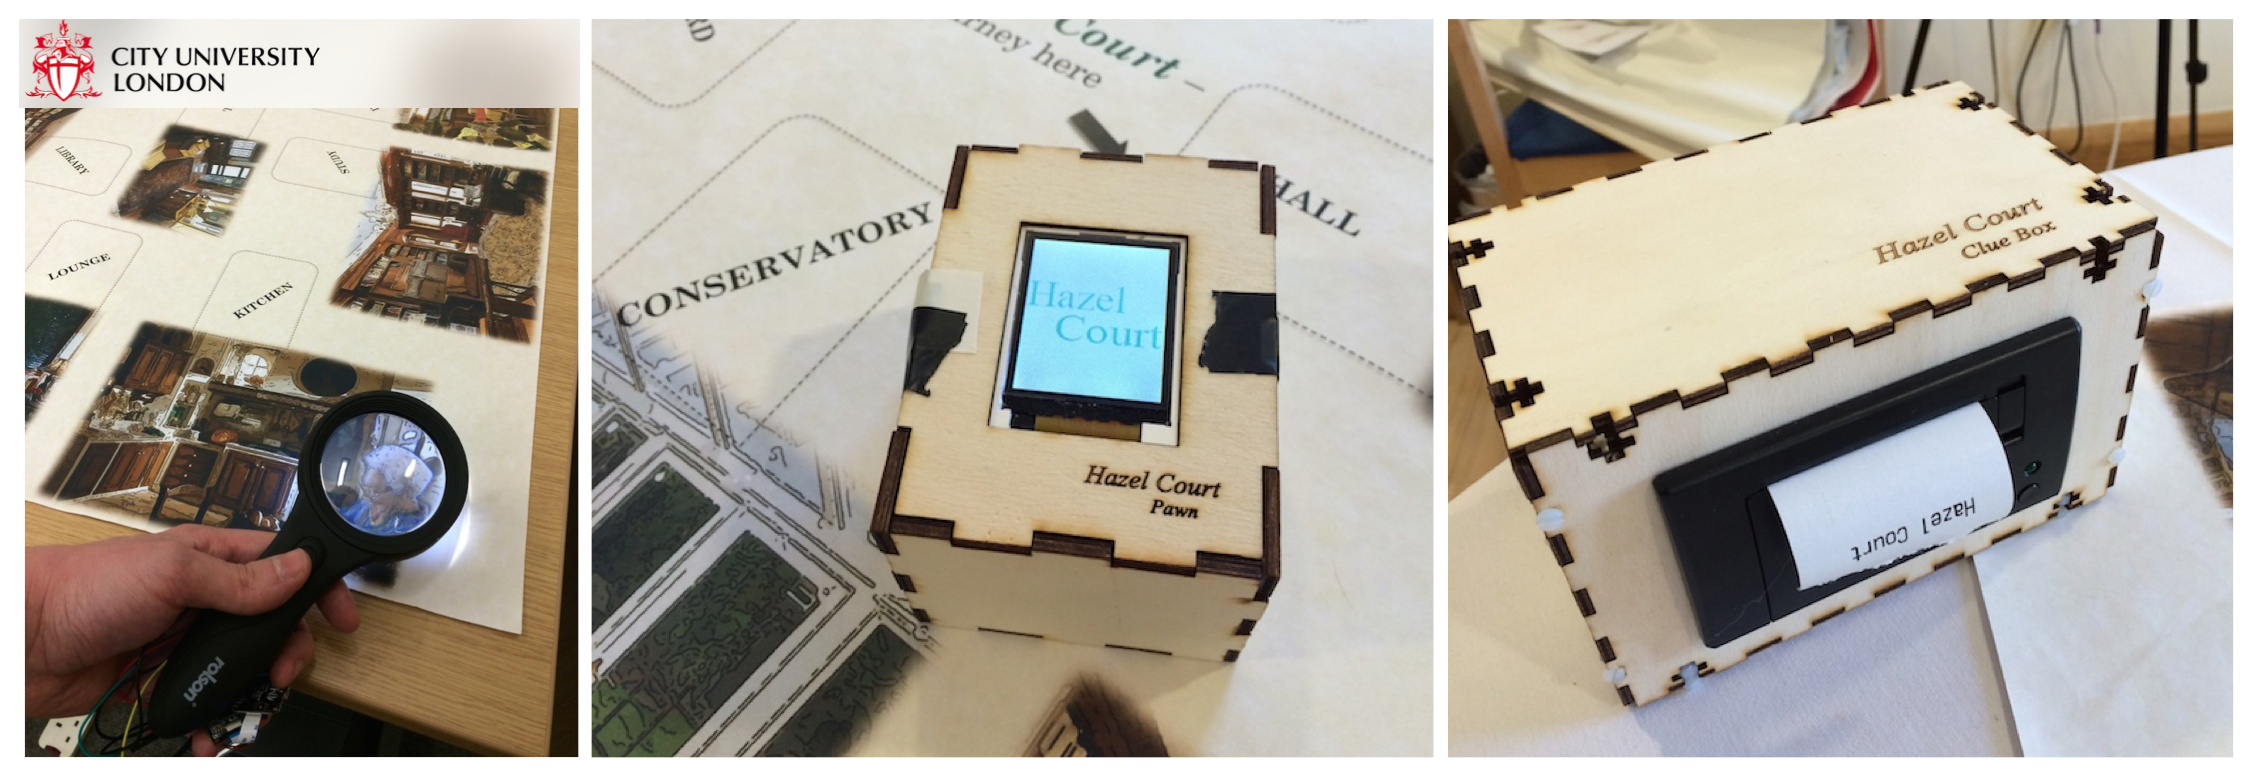
\includegraphics[width=1
	\textwidth]{city} \caption{The Hazel Court prototype} \label{fig:hazel-court} 
\end{figure}

During twelve weeks spent as visiting fellow at the MIT SENSEable City Lab I investigated the design and production of a tangible interface to promote user engagement and reflection about urban-mobility data. I worked under the supervision of professor Carlo Ratti. A working prototype of \emph{DriveWAVE} (Figure \ref{fig:drivewave}) has been implemented. DriveWAVE is a tangible interface that allows casual players in public spaces to challenge a computer brain against managing car flows towards minimizing pollution and avoiding traffic jams. The installation aims at sparking the interest in future sustainable cities\footnote{For more information please visit http://senseable.mit.edu/wave/}. The prototype features sensing-based interaction with the audience via presence sensors, physical controllers and digital projections. The work has been displayed to the public in two exhibitions: ``Wave'' held in Paris and ``CNR Internet Festival'' held in Pisa, Italy. This experiences streghtned my competences in building complex sensing-based systems to be deployed in public settings and added to the investigation of RQ3.
\begin{figure}
	[h] \centering 
	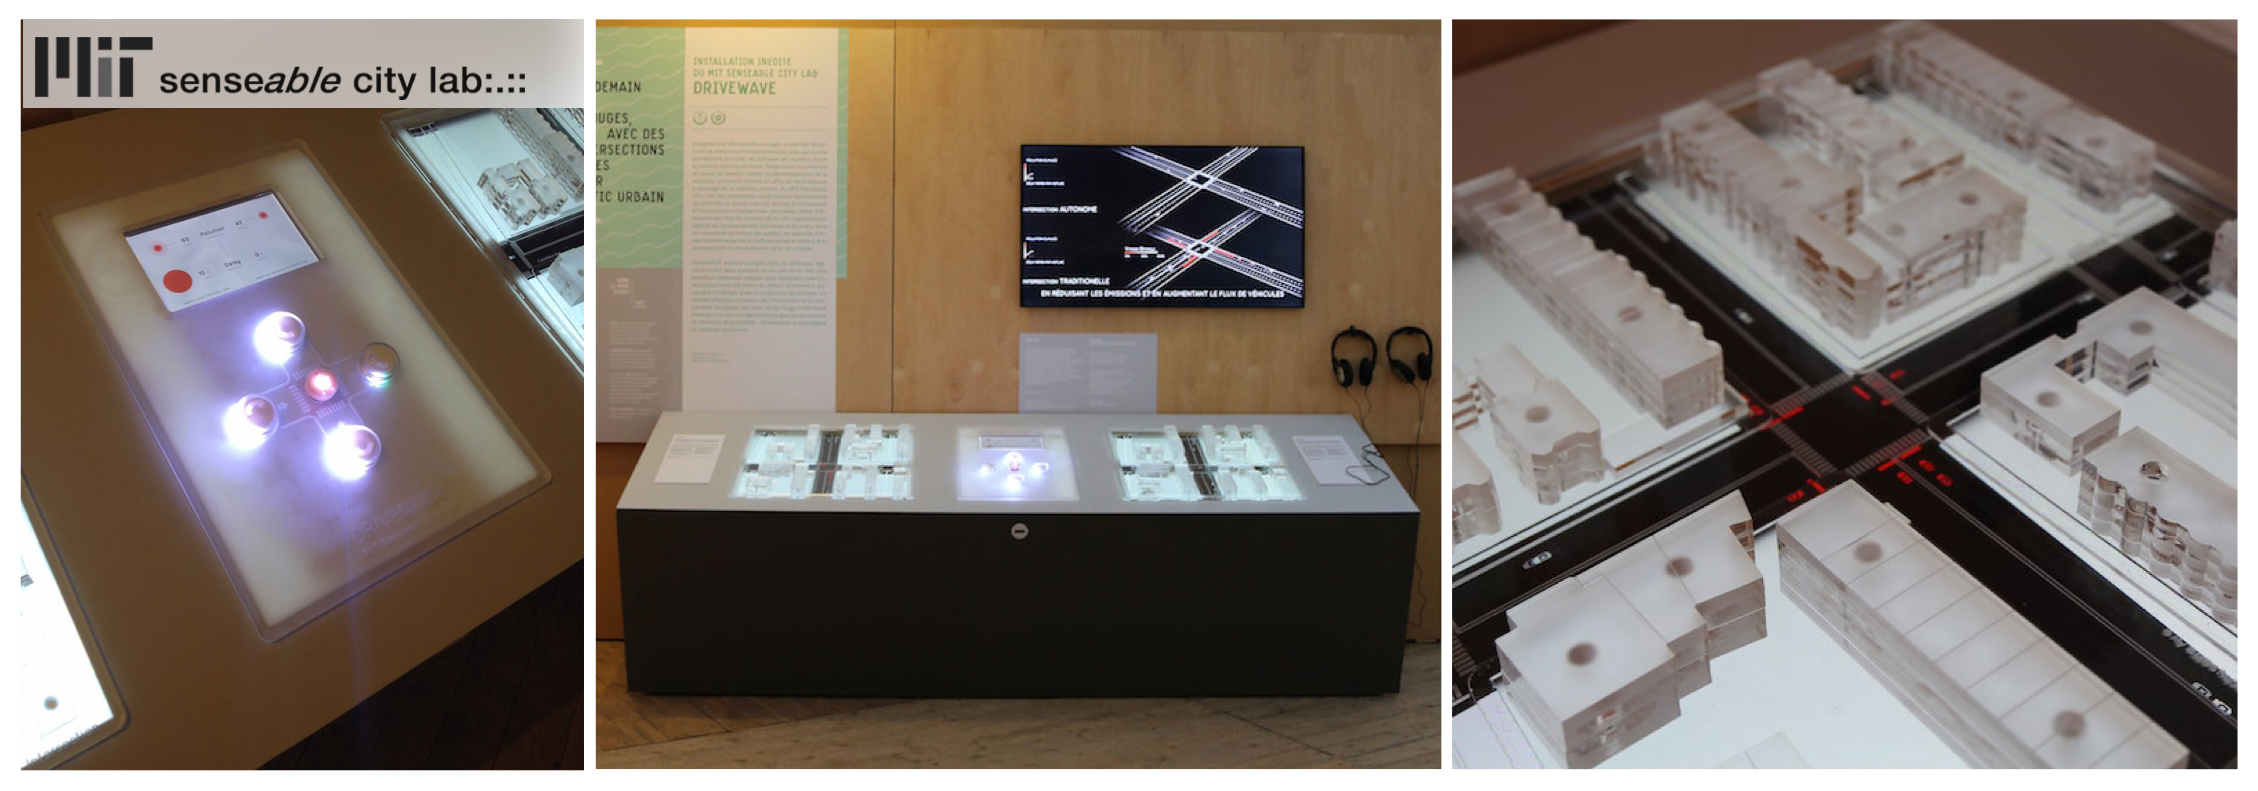
\includegraphics[width=1
	\textwidth]{mit} \caption{The DiveWAVE prototype} \label{fig:drivewave} 
\end{figure}
\chapter{Toolkits for rapid prototyping of sensing-based interfaces} \label{toolkits}

This appendix catalogue selected toolkits to ease prototyping of hardware and software features of sensing-based interfaces. A toolkit usually is composed by a mix of electronic circuitries, components, software libraries and communities of users willing to share knowledge and reveals implementation details of prototypes being built. 

The list reported in Table \ref{tab:toolkits} has been used to select relevant tools used to build the prototypes developed during the PhD work and can be used to drive future design iterations.  The toolkits hereafter reported has been selected after surveying, and in some case trying out, development tools either already available as commercial products or being available to beta testers. 

Toolkits are classified along four dimensions, chosen to support  challenges and requirements commonly found in the development of sensing-based interfaces:

\begin{itemize}
	\item \textbf{Modularity: }whether the tool allows to build transient electronic circuitries without requiring soldering or high expertise in electronic engineering. For example by means of wired or wireless plug-and-play modules. 
	\item \textbf{Connectivity: }whether the tool allows to effortlessly build internet-enabled prototypes by embedding wireless transceivers operating with standard protocols. For example providing ready to use bluetooth or wifi connectivity.
	\item \textbf{Ecology: }whether the tool provides guidelines and mechanisms to build applications that orchestrate a network of heterogeneous artefacts to provide a common functionality. For example to enable distributing user interaction on a number of different interfaces yet providing a consistent user experience.
	\item \textbf{Visual programming language: }whether the tools allows programming features using visual or other metaphors to speed up the development of software.
\end{itemize} 

In the following, Table \ref{tab:toolkits} details the toolkits reviewed. Rather than providing an exhaustive list of solutions the aim is at providing a reference to tools that somehow address the prototyping challenges found in this PhD work. 

%\begin{center}
	\begin{landscape}
	\begin{longtable}{P{2cm}P{1cm}P{1cm}P{1.5cm}P{1.5cm}P{1.5cm}P{.51cm}P{.51cm}}
	\caption[List of toolkits for rapid prototyping of sensing-based interfaces]{List of toolkits for rapid prototyping of sensing-based interfaces}	
     \label{tab:toolkits} \\

\hline
	    \multicolumn{1}{P{2cm}}{\textbf{Name}}  & \multicolumn{1}{P{1.5cm}}{\textbf{Price}}  & \multicolumn{1}{P{1.5cm}}{\textbf{Released}} & \multicolumn{1}{P{1.5cm}}{\textbf{Open\protect\newline source}} & \multicolumn{1}{P{1.5cm}}{\textbf{Modul.}}       & \multicolumn{1}{P{1.5cm}}{\textbf{Connect.}}           & \multicolumn{1}{P{1.5cm}}{\textbf{Ecology}} & \multicolumn{1}{P{1.5cm}}{\textbf{Visual\newline language}}                      \\ \midrule    
		
\endfirsthead
	    \multicolumn{1}{P{2cm}}{\textbf{Name}}  & \multicolumn{1}{P{1.5cm}}{\textbf{Price}}  & \multicolumn{1}{P{1.5cm}}{\textbf{Released}} & \multicolumn{1}{P{1.5cm}}{\textbf{Open\protect\newline source}} & \multicolumn{1}{P{1.5cm}}{\textbf{Modul.}}       & \multicolumn{1}{P{1.5cm}}{\textbf{Connect.}}           & \multicolumn{1}{P{1.5cm}}{\textbf{Ecology}} & \multicolumn{1}{P{1.5cm}}{\textbf{Visual\newline language}}                      \\ \midrule    
\endhead
\hline \multicolumn{8}{r}{{Continued on next page}} \\ \hline
\endfoot
\hline \hline
\endlastfoot
	    Arduino [1]                          & \$30     & 2005         & yes         &yes (tinker kit)  & yes (w/extra hw)   & no   & yes (ardublock)  \\
	    RaspberryPi [2]                      & \$40      & 2012         & yes         & no               & yes \newline(w/extra hw)    & no      & yes \newline (scratch)         \\
	    LittleBits [3]                        & \$100 & 2008         & yes         & yes              & yes (wifi)             & no      & no                                \\
	    Lightblue Bean [4]                    & \$30      & 2013         & partially   & no               & yes (ble)              & no      & no                      \\
	    Printoo [5]                           & \$45    & 2014         & yes         & yes              & yes (ble)              & no      & no                       \\
	    Bitalino [6]                          & \$45          & 2014         & n/a         & yes              & n/a                    & no      & no                                \\
	    Atomwear [7]                          & \$45   & 2014         & yes         & yes              & yes (ble)              & no      & no                   \\
	    Microduino [8]                        & \$20         & 2013         & yes         & yes              & yes (BT)               & no      & no                       \\
	    Twine [9]                             & \$99        & 2012         & n/a         & no               & yes (wifi)             & no      & no                                \\
	    Microview [10]                         & \$45        & 2014         & partially   & no               & no                     & no      & no                       \\
	    Xadow [11]                             & \$30        & 2012         & no          & yes              & yes (ble)              & no      & no                      \\
	    Kano Computer [12]                      & \$99        & 2013         & partially   & no               & yes (wifi)             & no      & yes\newline (scratch)                     \\
	    Spark [13]                             & \$39       & 2013         & partially   & no               & yes (wifi)             & no      & no                 \\
	    Wonderbar [14]                          & \$100 & 2013         & no          & yes              & yes (ble+wifi)         & n/a     & yes              \\
	    Metawear [15]                          & \$35   & 2014         & no          & no               & yes (ble)              & no      & no                         \\
	    Smart Citizen [16]                      & \$100  & 2012         & no          & partially        & yes (wifi)             & no      & no                                \\
	    Circuit Scribe [17]                    & \$30   & 2014         & no          & yes              & no                     & no      & no                                \\
	    Verve 2 [18]                           & \$45   & 2014         & n/a         & yes              & no                     & no      & n/a                               \\
	    Notion	[19]						   & \$99        & 2014         & no          & yes              & no                     & no      & no             \\
	    Make!Sense [20]                        & \$39        & 2014         & no          & yes              & no                     & no      & yes\newline (scratch)                     \\
	    McThings [21]                          & \$100       & 2014         & n/a         & yes              & yes (ble+wifi)         & no      & yes            \\
	    Gadgeteer [22]                         & \$100   & 2009         & no          & no               & no                     & no      & no                                \\
	    Intel Edison\newline Sparkfun Blocks [23]     & \$120   & 2015         & no          & yes              & yes (ble+wifi)         & no      & no                                \\
	    Mesh [24]                              & \$105   & 2015         & n/a         & yes              & yes (ble)              & yes     & yes                               \\
	    Spark Photon [25]                       & \$19        & 2015         & n/a         & no               & yes (wifi)             & no      & no                                \\
	    Airboard [26]                          & \$20        & 2015         & no          & yes              & yes                    & no      & no                                \\
	    HIRIS [27]                             & \$100       & 2015         & n/a         & yes              & yes(ble)               & no      & no                                \\				
	\bottomrule
	\end{longtable}
	\end{landscape}
	
	\textbf{References: }
	
	[1]: http://arduino.cc  \newline
	[2]: http://raspberrypi.org  \newline
	[3]: http://littlebits.cc  \newline
	[4]: http://punchthrough.com/bean/ \newline
	[5]: http://printoo.pt \newline
	[6]: http://www.bitalino.com/ \newline
	[7]: https://www.kickstarter.com/projects/343910040/atomwear \newline
	[8]: https://www.kickstarter.com/projects/microduino/microduino-arduino-in-your-pocket-small-stackable \newline
	[9]: https://www.kickstarter.com/projects/supermechanical/twine-listen-to-your-world-talk-to-the-internet \newline
	[10]: https://www.kickstarter.com/projects/1516846343/microview-chip-sized-arduino-with-built-in-oled-di \newline
	[11]: http://www.seeedstudio.com/depot/s/xadow.html \newline
	[12]: https://www.kickstarter.com/projects/alexklein/kano-a-computer-anyone-can-make \newline
	[13]: https://www.kickstarter.com/projects/sparkdevices/spark-core-wi-fi-for-everything-arduino-compatible \newline
	[14]: http://www.dragoninnovation.com/projects/35-wunderbar-by-relayr \newline
	[15]: https://www.kickstarter.com/projects/guardyen/metawear-production-ready-wearables-in-30-minutes  \newline
	[16]: https://www.kickstarter.com/projects/acrobotic/the-smart-citizen-kit-crowdsourced-environmental \newline
	[17]: https://www.kickstarter.com/projects/electroninks/circuit-scribe-draw-circuits-instantly \newline
	[18]: https://www.kickstarter.com/projects/54060271/verve2-connect-your-world-to-your-computer-and-int \newline
	[19]: https://www.kickstarter.com/projects/1044009888/notion-be-home-even-when-youre-not \newline
	[20]: https://www.kickstarter.com/projects/1978340629/makesense-a-universal-interface-for-learning \newline
	[21]: https://www.kickstarter.com/projects/2016620887/mcthings-tiny-wireless-bluetooth-sensors-and-contr \newline
	[22]: http://www.netmf.com/gadgeteer/ \newline
	[23]: https://www.sparkfun.com/products/13276 \newline
	[24]: https://www.indiegogo.com/projects/mesh-creative-diy-kit-for-the-connected-life \newline
	[25]: https://www.spark.io \newline
	[26]: https://www.kickstarter.com/projects/223628811/the-airboard-sketch-internet-of-things-fast  \newline
	[27]: https://www.indiegogo.com/projects/hiris-the-first-wearable-computer-for-everyone \newline

	
%	\end{center}








\backmatter
\printbibliography

\end{document}